\section{Test plan} \label{sec:test}

In the early stage, testing and verification of the algorithms and retrieval system are vital. While the retrieval system is completed, some test cases are also important to evaluate the performance of the system. A series of tests are carried out:

\begin{enumerate}[1.]
\item Retrieval test
\item Rotation invariant test
\item Noise resistant test
\item ``Scan to search'' test
\item Large database test
\end{enumerate}

The first step is to test that the retrieval system can operate correctly. A model from the model database will be input to the search engine to retrieve. The result is expected to find the model which is exact the same as the input one. 

The second step is to verify the descriptors are correctly computed, i.e., the rotational invariance property of the descriptors is shown. A model from the model database will be loaded, and a random rotation will be applied to the model. Then this model is queried in the system. The best result is finding out exact the same model from the database. However, due to the potential error of coefficients in rotation or rasterization, if the system shows models with similar shape, the system can still be decided as robust. 

The third step is to test the denoising module and verify the noise resistant property of the system. A model from the model database will be loaded and noise will be added. Then the denoising function is called. As the denoise module and the rasterization module cannot perfectly eliminate the noise, the system can be decided as robust if the query result shows models with same or similar shapes. 

If the first three tests are passed, the pre-processing modules and the matching algorithm are considered to be correctly implemented. Afterwards, ``Scan to search'' test can be carried out. The scanned model is loaded and denoised. Then the model is queried in the system. The results will indicate how well the matching algorithm works. The last test is to verify the system's robustness to large database, where a large number of descriptors may have influence to the retrieval accuracy. 

\section{Test results} \label{sec:results}

\subsection{Retrieval test} 

The aim of this test is to make sure the retrieval system can operate successfully. As Figure~\ref{retrievaltest_UI} demonstrates, the test result indicates every module of the retrieval system is correctly implemented, and the models in the database can be retrieved. 

\subsection{Rotation invariant test} \label{sec:results_rotationinvarianttest}

There are two test cases in this test. The first is to input a rotated model with a cylinder-like shape and search. The input and output are demonstrated in Figure~\ref{noiseinvarianttest_UI1}. The first candidate model (with the highest similarity) has exactly the same shape as the input model. Two types of descriptors of the rotated model and the matched model are analised and plotted(Figure~\ref{rotationinvarianttest_analysis1}). Comparing with the rotated model and the origin model, their spherical harmonics descriptors have almost the same feature in 2D, and their distance histogram descriptors have almost the same feature in 1D. Thus the rotation invariant property of the two descriptors is verified.

In the second test, a flat model is rotated and queried. This is to test the robustness of the descriptors against any rotated shape. Figure~\ref{noiseinvarianttest_UI2} demonstrates the input and output. Also, the same model is found. However, the analysis of the descriptors (Figure~\ref{rotationinvarianttest_analysis2}) shows that there is an unusual burst in the spherical harmonics descriptors of the rotated model(located in radius range 12 to 13). It is perhaps caused by the sampling error in rasterization. But with the assistance of the distance histogram descriptors, whose statistical feature almost have no difference in this case, the final matching result is still satisfactory. 

\subsection{Noise resistant test}

Some noise is generated by the noise generator and added to the model (Figure~\ref{noiseinvarianttest_UI} (a)). Then the denoising function is called(Figure~\ref{noiseinvarianttest_UI} (b)). With the bilateral filter, the sharp edges of the model are kept while the other parts are smoothed. And the query result shows candidate models (Figure~\ref{noiseinvarianttest_UI} (c)). The first candidate model (with the highest similarity) has the same shape as the input model. The descriptors of the denoised model and the matched model are analised and plotted (Figure~\ref{noiseinvarianttest_analysis}). Comparing with the noisy model and the origin model, two types of the shape descriptors have similar features but only some slight changes. Therefore the noise resistant property of this system is verified. 

\subsection{``Scan to search'' test}

A scanned ``engine'' model is created in Figure~\ref{scantosearchtest_engine_scanning}. Unwanted leftovers are removed from the raw model (Figure~\ref{scantosearchtest_engine_scanning} (b)). 
After searching, the output is in Figure~\ref{scantosearchtest_engine_UI}. Models that have similar shapes with the scanned ``engine'' model are found. 

Additionally, more ``Scan to search'' query tests are carried out. A manufacturing component, a bin and a single-board computer are scanned and their 3D models are created(Figure~\ref{scantosearchtest_component_scanning}, Figure~\ref{scantosearchtest_bin_scanning} and Figure~\ref{scantosearchtest_pi_scanning}). And the retrieval results are demonstrated in Figure~\ref{scantosearchtest_component_UI}, Figure~\ref{scantosearchtest_bin_UI} and Figure~\ref{scantosearchtest_pi_UI}.

\subsection{Large database test}

After testing the whole functions of the system, the database is expanded from 30 models size to 60 models size. This is to make sure there is no potential risk when the database is large. With the initial design, there is only one spherical harmonics descriptors. And a single type of descriptors may have its weakness. Due to some unknown errors in the descriptors (maybe it is the rasterization error or sampling error in the spherical harmonics decomposition. See the rotation invariant test 2 in Section~\ref{sec:results_rotationinvarianttest}), there are sometimes some irrelevant matches. This is also analysed in Section~\ref{sec:thefinaldesign}.  Therefore, another type of descriptors (distance histogram) is added for assistance and compensating the error caused by spherical harmonics. 

\section{Evaluation}

From all the tests, the results indicate that the performance of the matching algorithms (two descriptors: spherical harmonics and distance histogram) is satisfactory. Models with similar shapes can be found when the input model is noisy and rotated. In the final ``scan to search'' tests, the matched models also have similar shape features with the input scanned model. 

However, since the spherical harmonics decomposition has $O(n^3)$ computational complexity for cut-off frequency $n$, it is time-consuming to transform a model with a large amount of voxels (the average transformation time is 30 seconds). Also the spherical harmonics tend to have numerical errors in some circumstances (e.g. a model with unusual shape). Thus the distance histogram descriptors are introduced to compensate these errors. 

Besides, both type of the descriptors (spherical harmonics and distance histogram) have a same drawback. According to their features and properties, they cannot detect interior rotation of a model. 

\begin{figure}
\begin{center}
\begin{tabular}{cc}   % The "|" bar puts a bar in the figure
   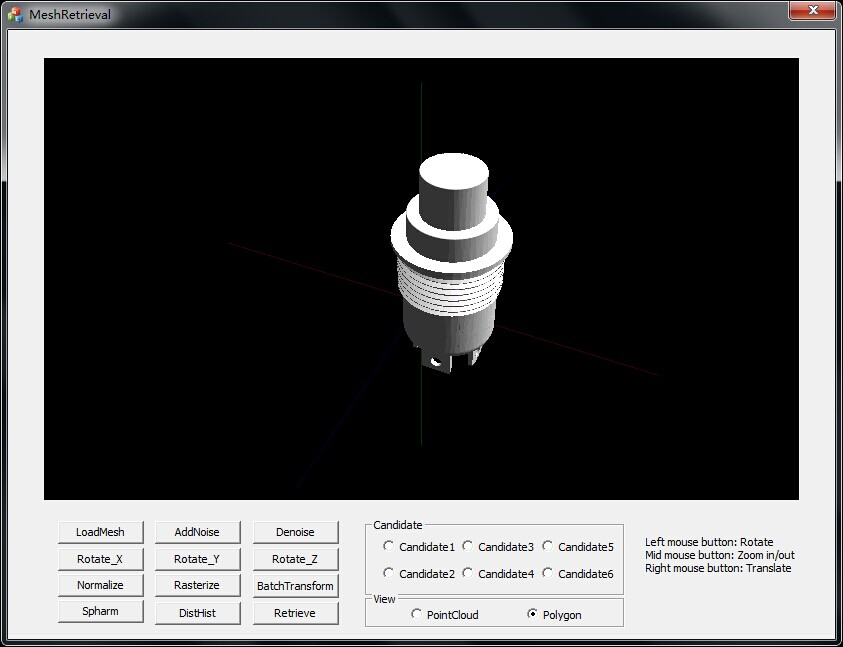
\includegraphics[width=0.6\linewidth]{input_initialdesign}  \\
   (a)\\
\end{tabular}
   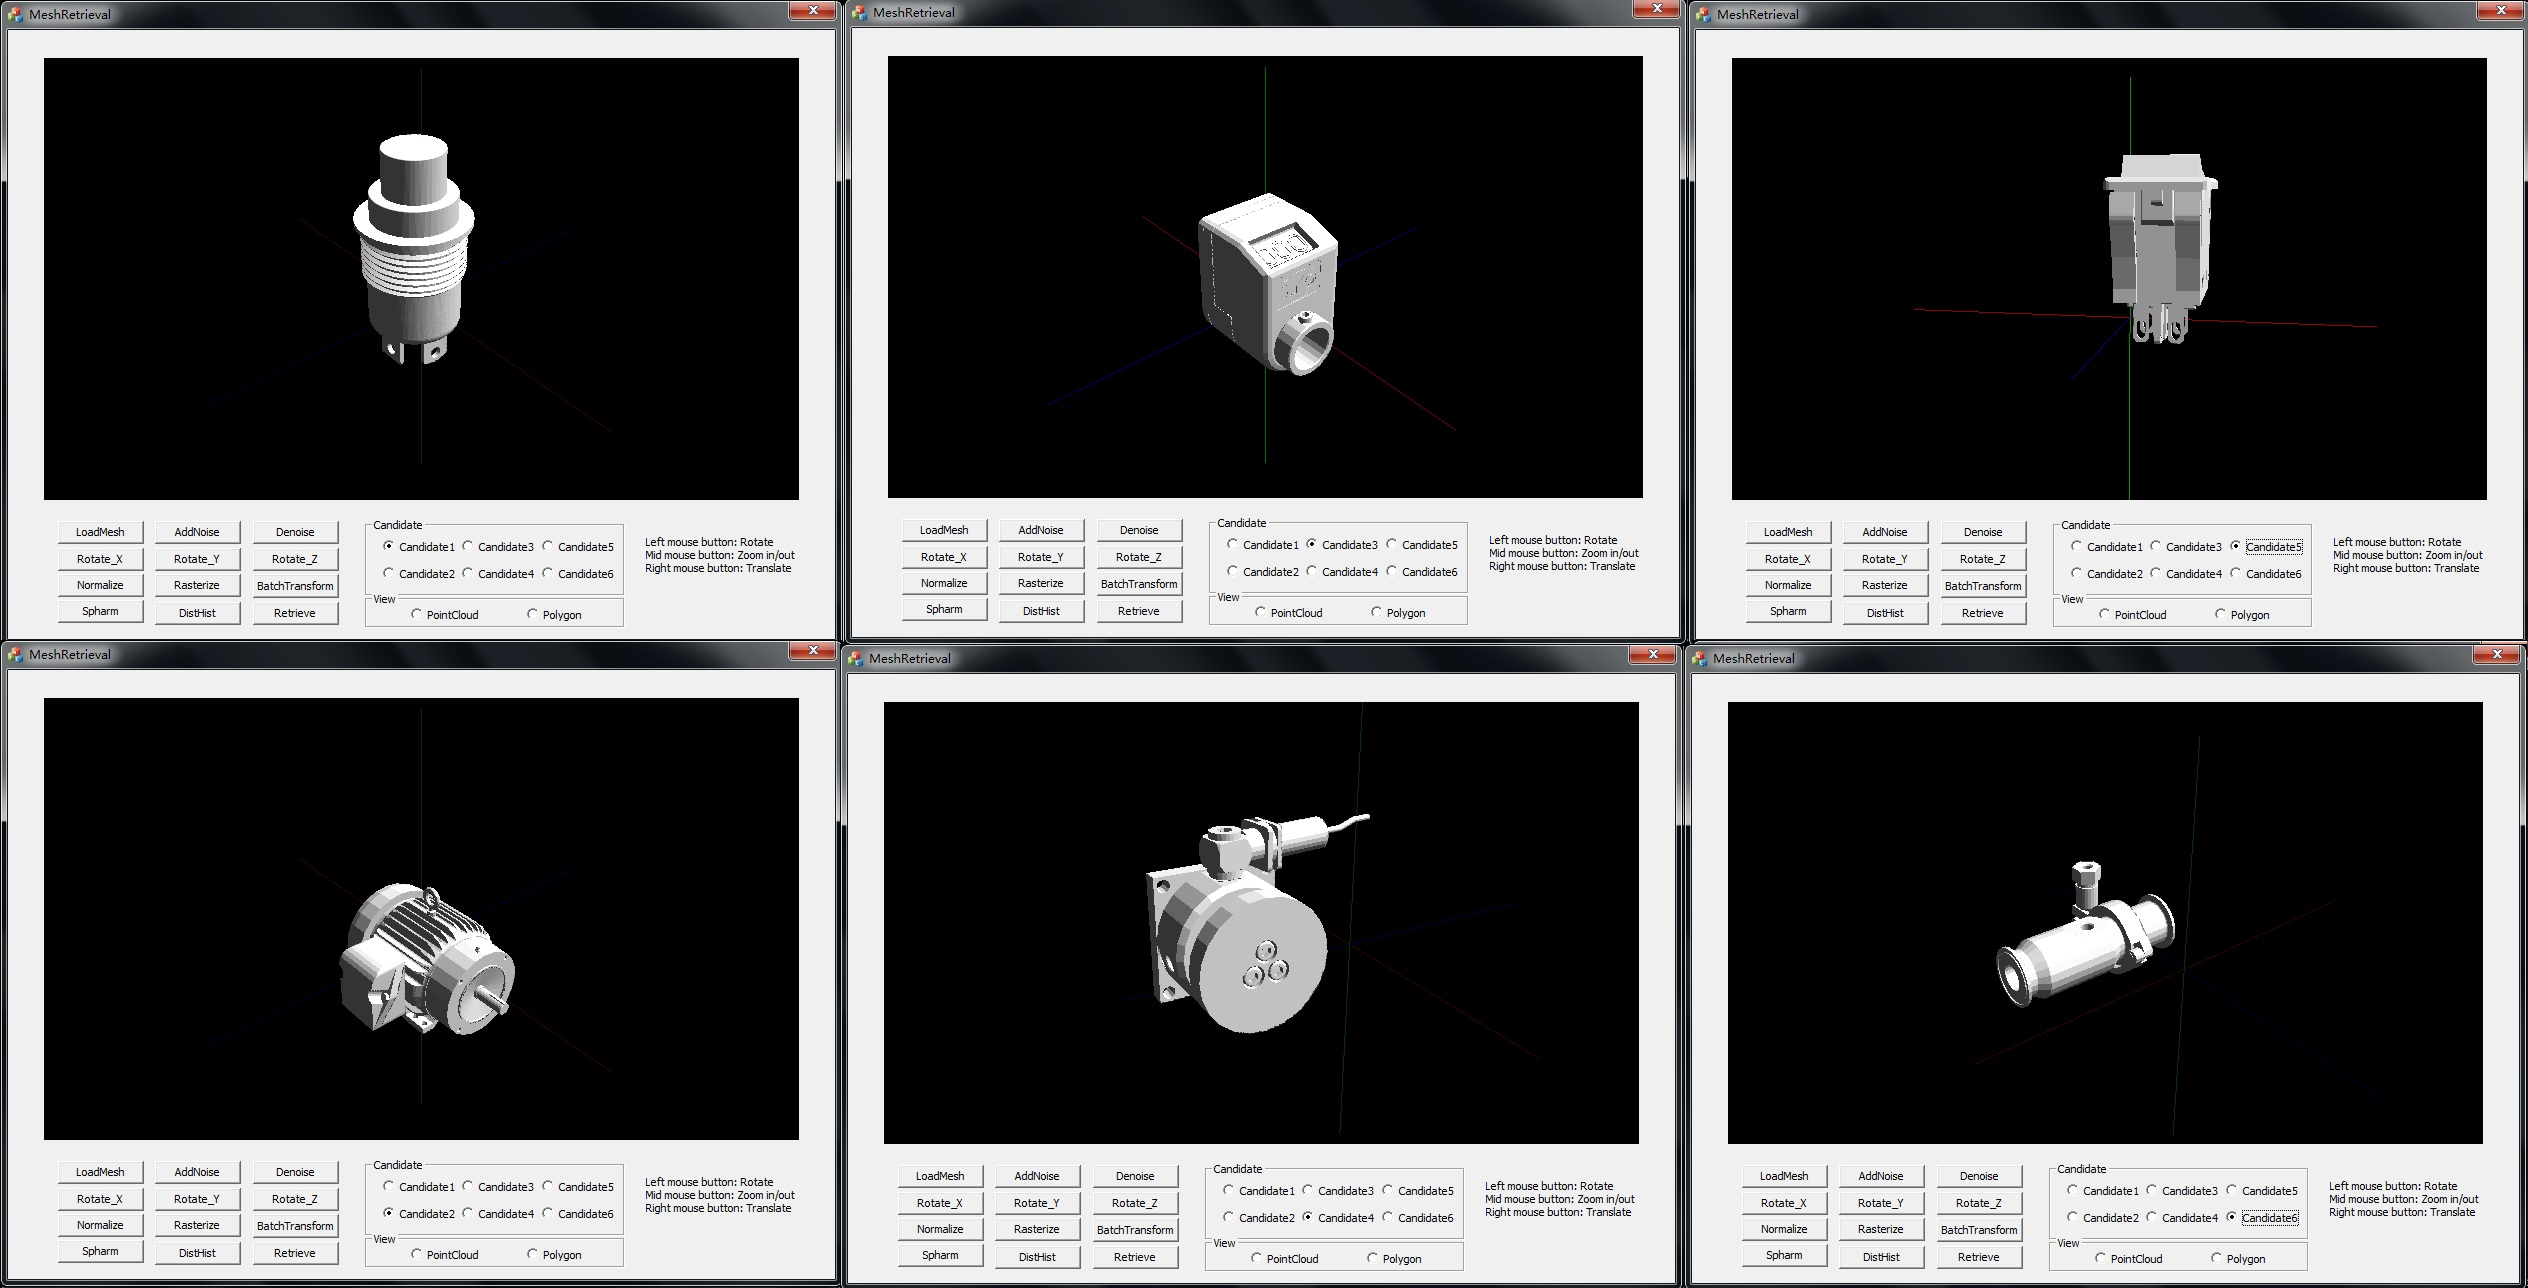
\includegraphics[width=1\linewidth]{output_finaldesign}  \\
   (b)\\
\caption{Retrieval test: (a) the input model. (b) the query result. The result indicates every module of the retrieval system is correctly implemented, and the models in the database can be retrieved successfully.} 
  \label{retrievaltest_UI}
\end{center}
\end{figure}

\begin{figure}
\begin{center}
\begin{tabular}{cc}   % The "|" bar puts a bar in the figure
   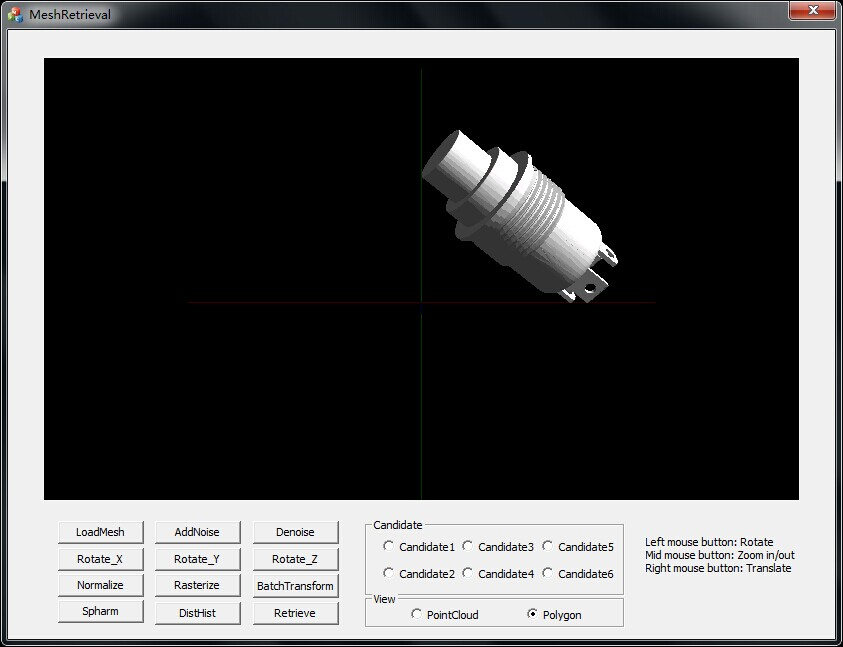
\includegraphics[width=0.6\linewidth]{input_rotationinvariant_test10}  \\
   (a) \\
\end{tabular}
   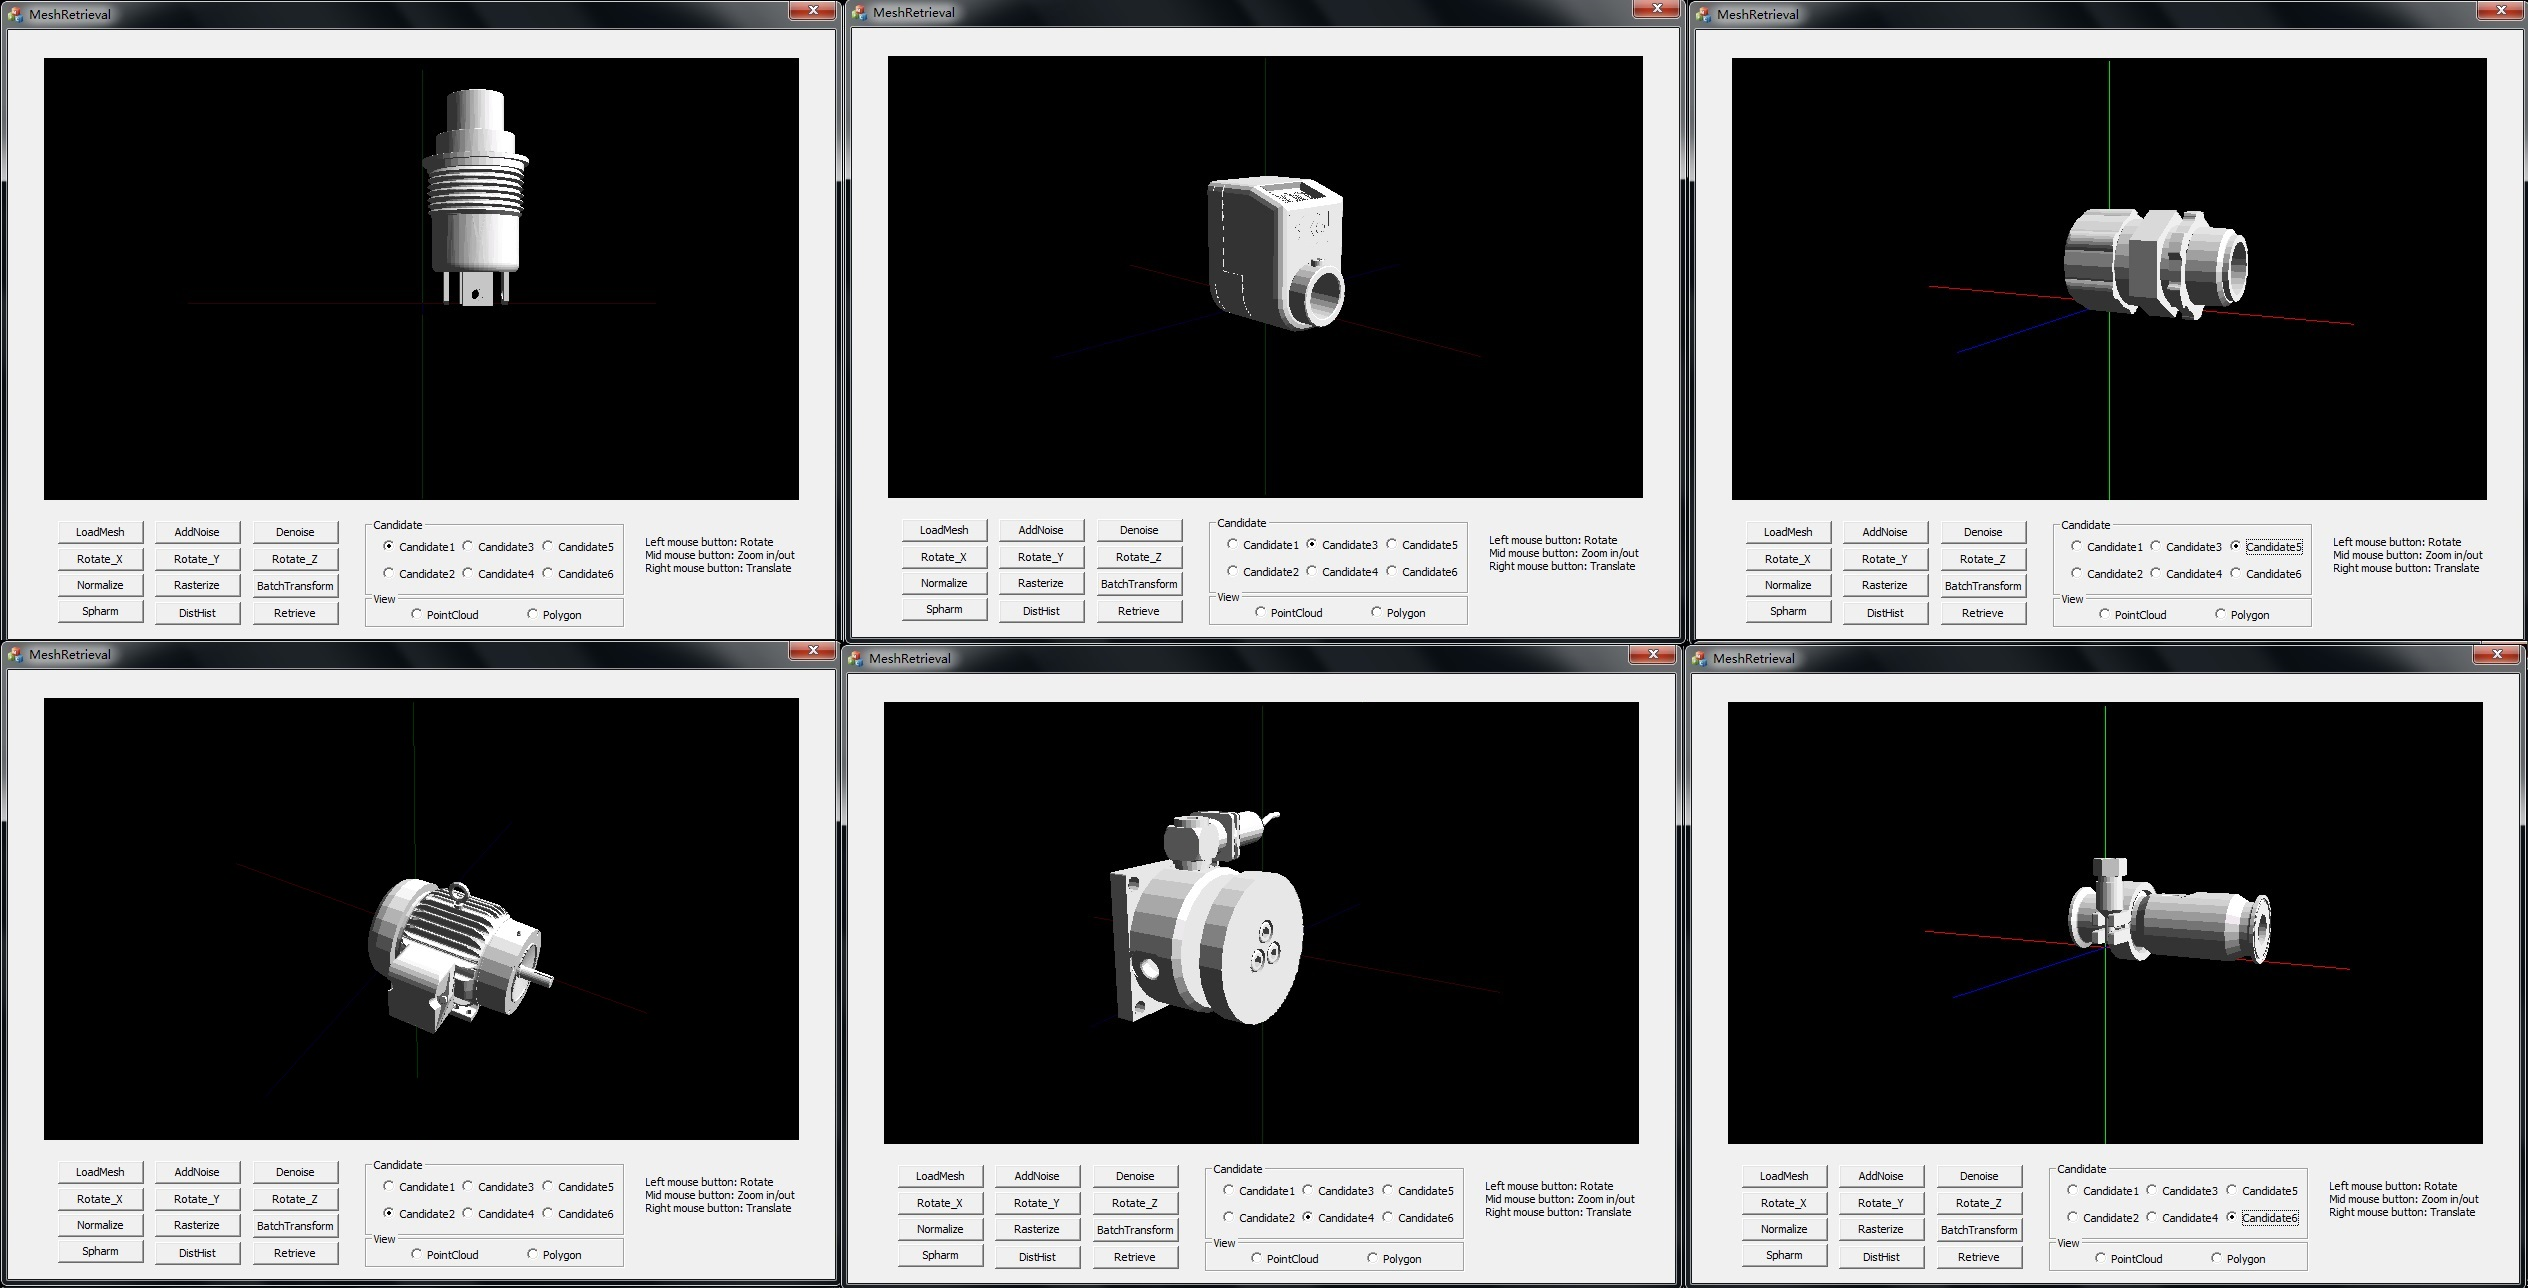
\includegraphics[width=1\linewidth]{output_rotationinvariant_test10}  \\
   (b)  \\
\caption{Rotation invariant test 1: (a) the input model (rotated). (b) the query result. It can be noticed that the first candidate model has the same shape as the input model.} 
  \label{noiseinvarianttest_UI1}
\end{center}
\end{figure}

\begin{figure}
\begin{center}
\begin{tabular}{cc}   % The "|" bar puts a bar in the figure
   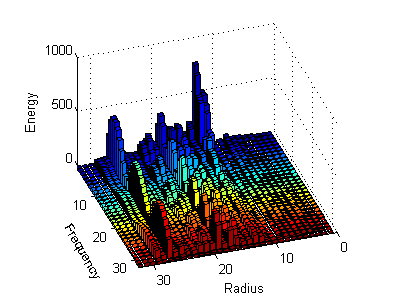
\includegraphics[width=0.45\linewidth]{rotationinvariant_test_SH10_rotated} & 
   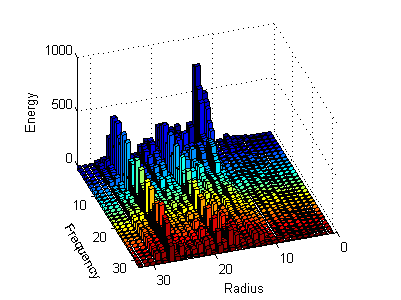
\includegraphics[width=0.45\linewidth]{rotationinvariant_test_SH10_origin}  \\
   (a) Spherical harmonics (rotated model) & (b) Spherical harmonics (origin model) \\
   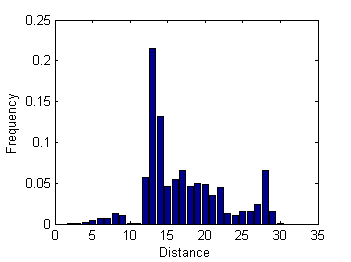
\includegraphics[width=0.45\linewidth]{rotationinvariant_test_DH10_rotated} &
   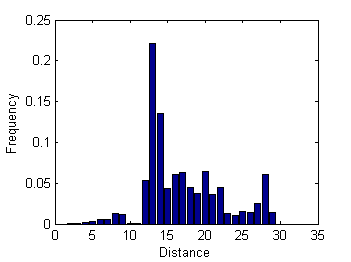
\includegraphics[width=0.45\linewidth]{rotationinvariant_test_DH10_origin}  \\
   (c) Distance histogram (rotated model) & (d) Distance histogram (origin model)\\
\end{tabular}
\caption{Analysis of the rotation invariant test 1: (a) and (b) have almost the same statistical distribution, (c) and (d) have almost the same statistical distribution. Thus the rotation invariant property of the two descriptors is verified.} 
  \label{rotationinvarianttest_analysis1}
\end{center}
\end{figure}

\begin{figure}
\begin{center}
\begin{tabular}{cc}   % The "|" bar puts a bar in the figure
   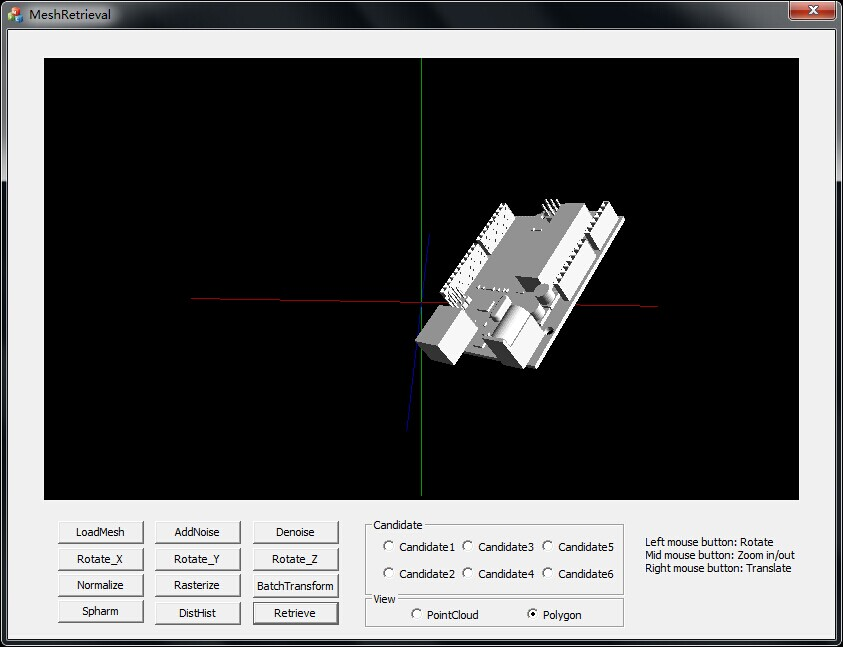
\includegraphics[width=0.6\linewidth]{input_rotationinvariant_test32}  \\
   (a) \\
\end{tabular}
   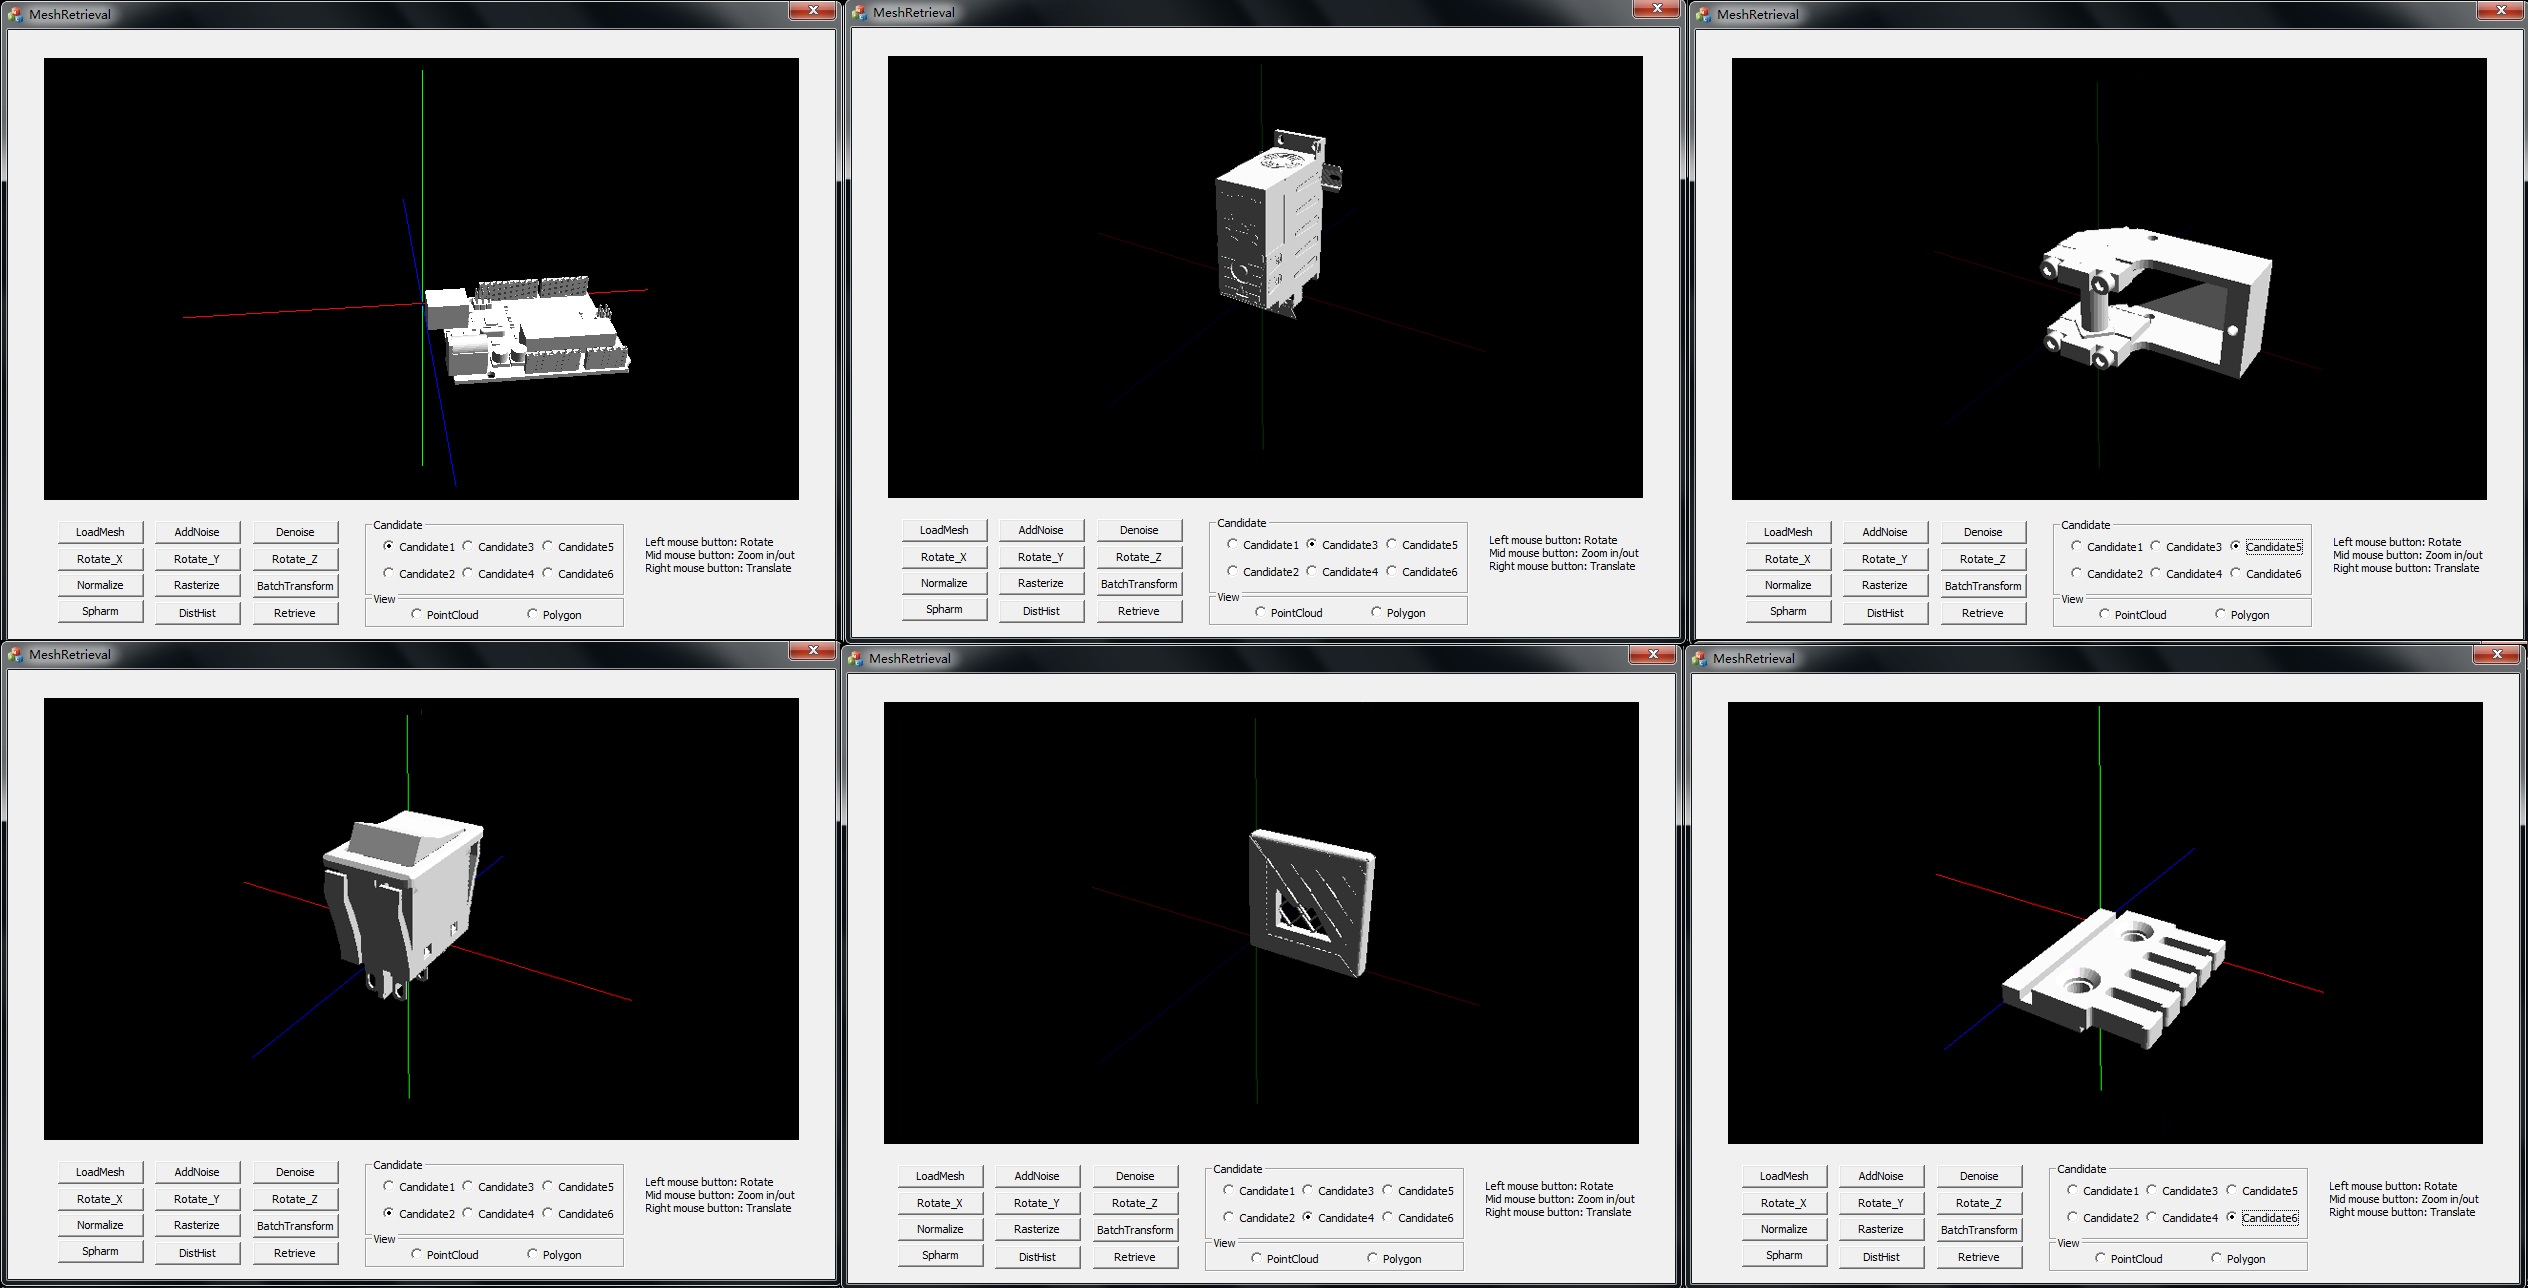
\includegraphics[width=1\linewidth]{output_rotationinvariant_test32}  \\
   (b)  \\
\caption{Rotation invariant test 2: (a) the input model (rotated). (b) the query result. It can be noticed that the first candidate model has the same shape as the input model.} 
  \label{noiseinvarianttest_UI2}
\end{center}
\end{figure}

\begin{figure}
\begin{center}
\begin{tabular}{cc}   % The "|" bar puts a bar in the figure
   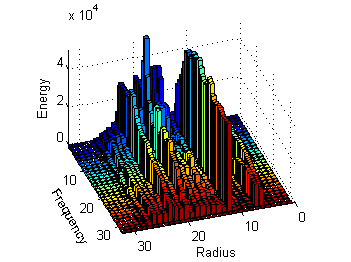
\includegraphics[width=0.45\linewidth]{rotationinvariant_test_SH32_rotated} & 
   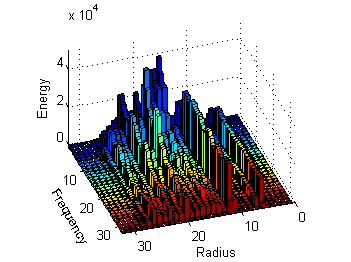
\includegraphics[width=0.45\linewidth]{rotationinvariant_test_SH32_origin}  \\
   (a) Spherical harmonics (rotated model) & (b) Spherical harmonics (origin model) \\
   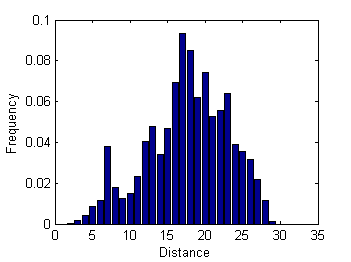
\includegraphics[width=0.45\linewidth]{rotationinvariant_test_DH32_rotated} &
   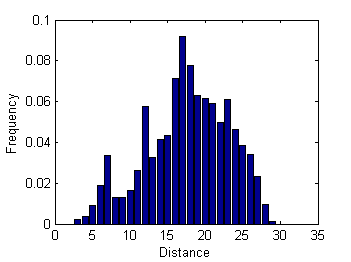
\includegraphics[width=0.45\linewidth]{rotationinvariant_test_DH32_origin}  \\
   (c) Distance histogram (rotated model) & (d) Distance histogram (origin model)  \\
\end{tabular}
\caption{Analysis of the rotation invariant test 2: Comparing with (a) and (b), there is an unusual burst in (a) (located in radius range 12 to 13). It is perhaps caused by the sampling error in rasterization. 
With the assistance of (c), whose statistical feature almost have no difference with (d), the final matching result is still satisfactory.} 
  \label{rotationinvarianttest_analysis2}
\end{center}
\end{figure}


\begin{figure}
\begin{center}
\begin{tabular}{cc}   % The "|" bar puts a bar in the figure
   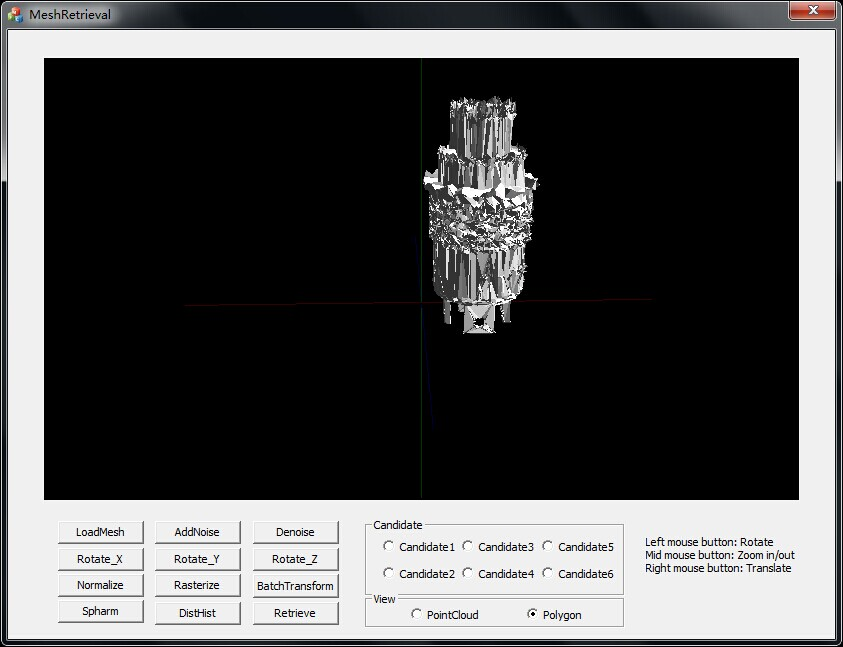
\includegraphics[width=0.45\linewidth]{input_noiseinvariant_test_addnoise10} & 
   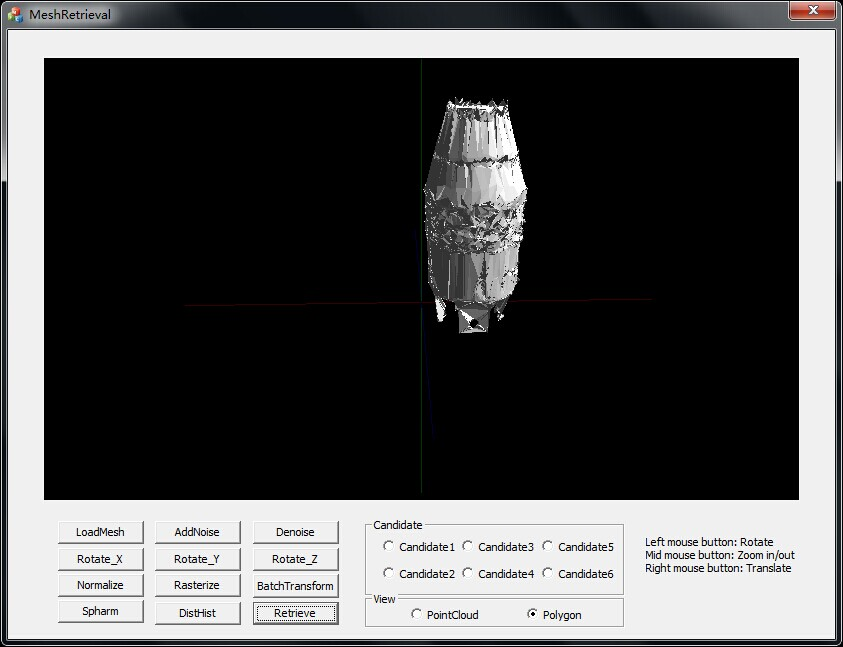
\includegraphics[width=0.45\linewidth]{input_noiseinvariant_test_denoise10}  \\
   (a) & (b) \\
\end{tabular}
   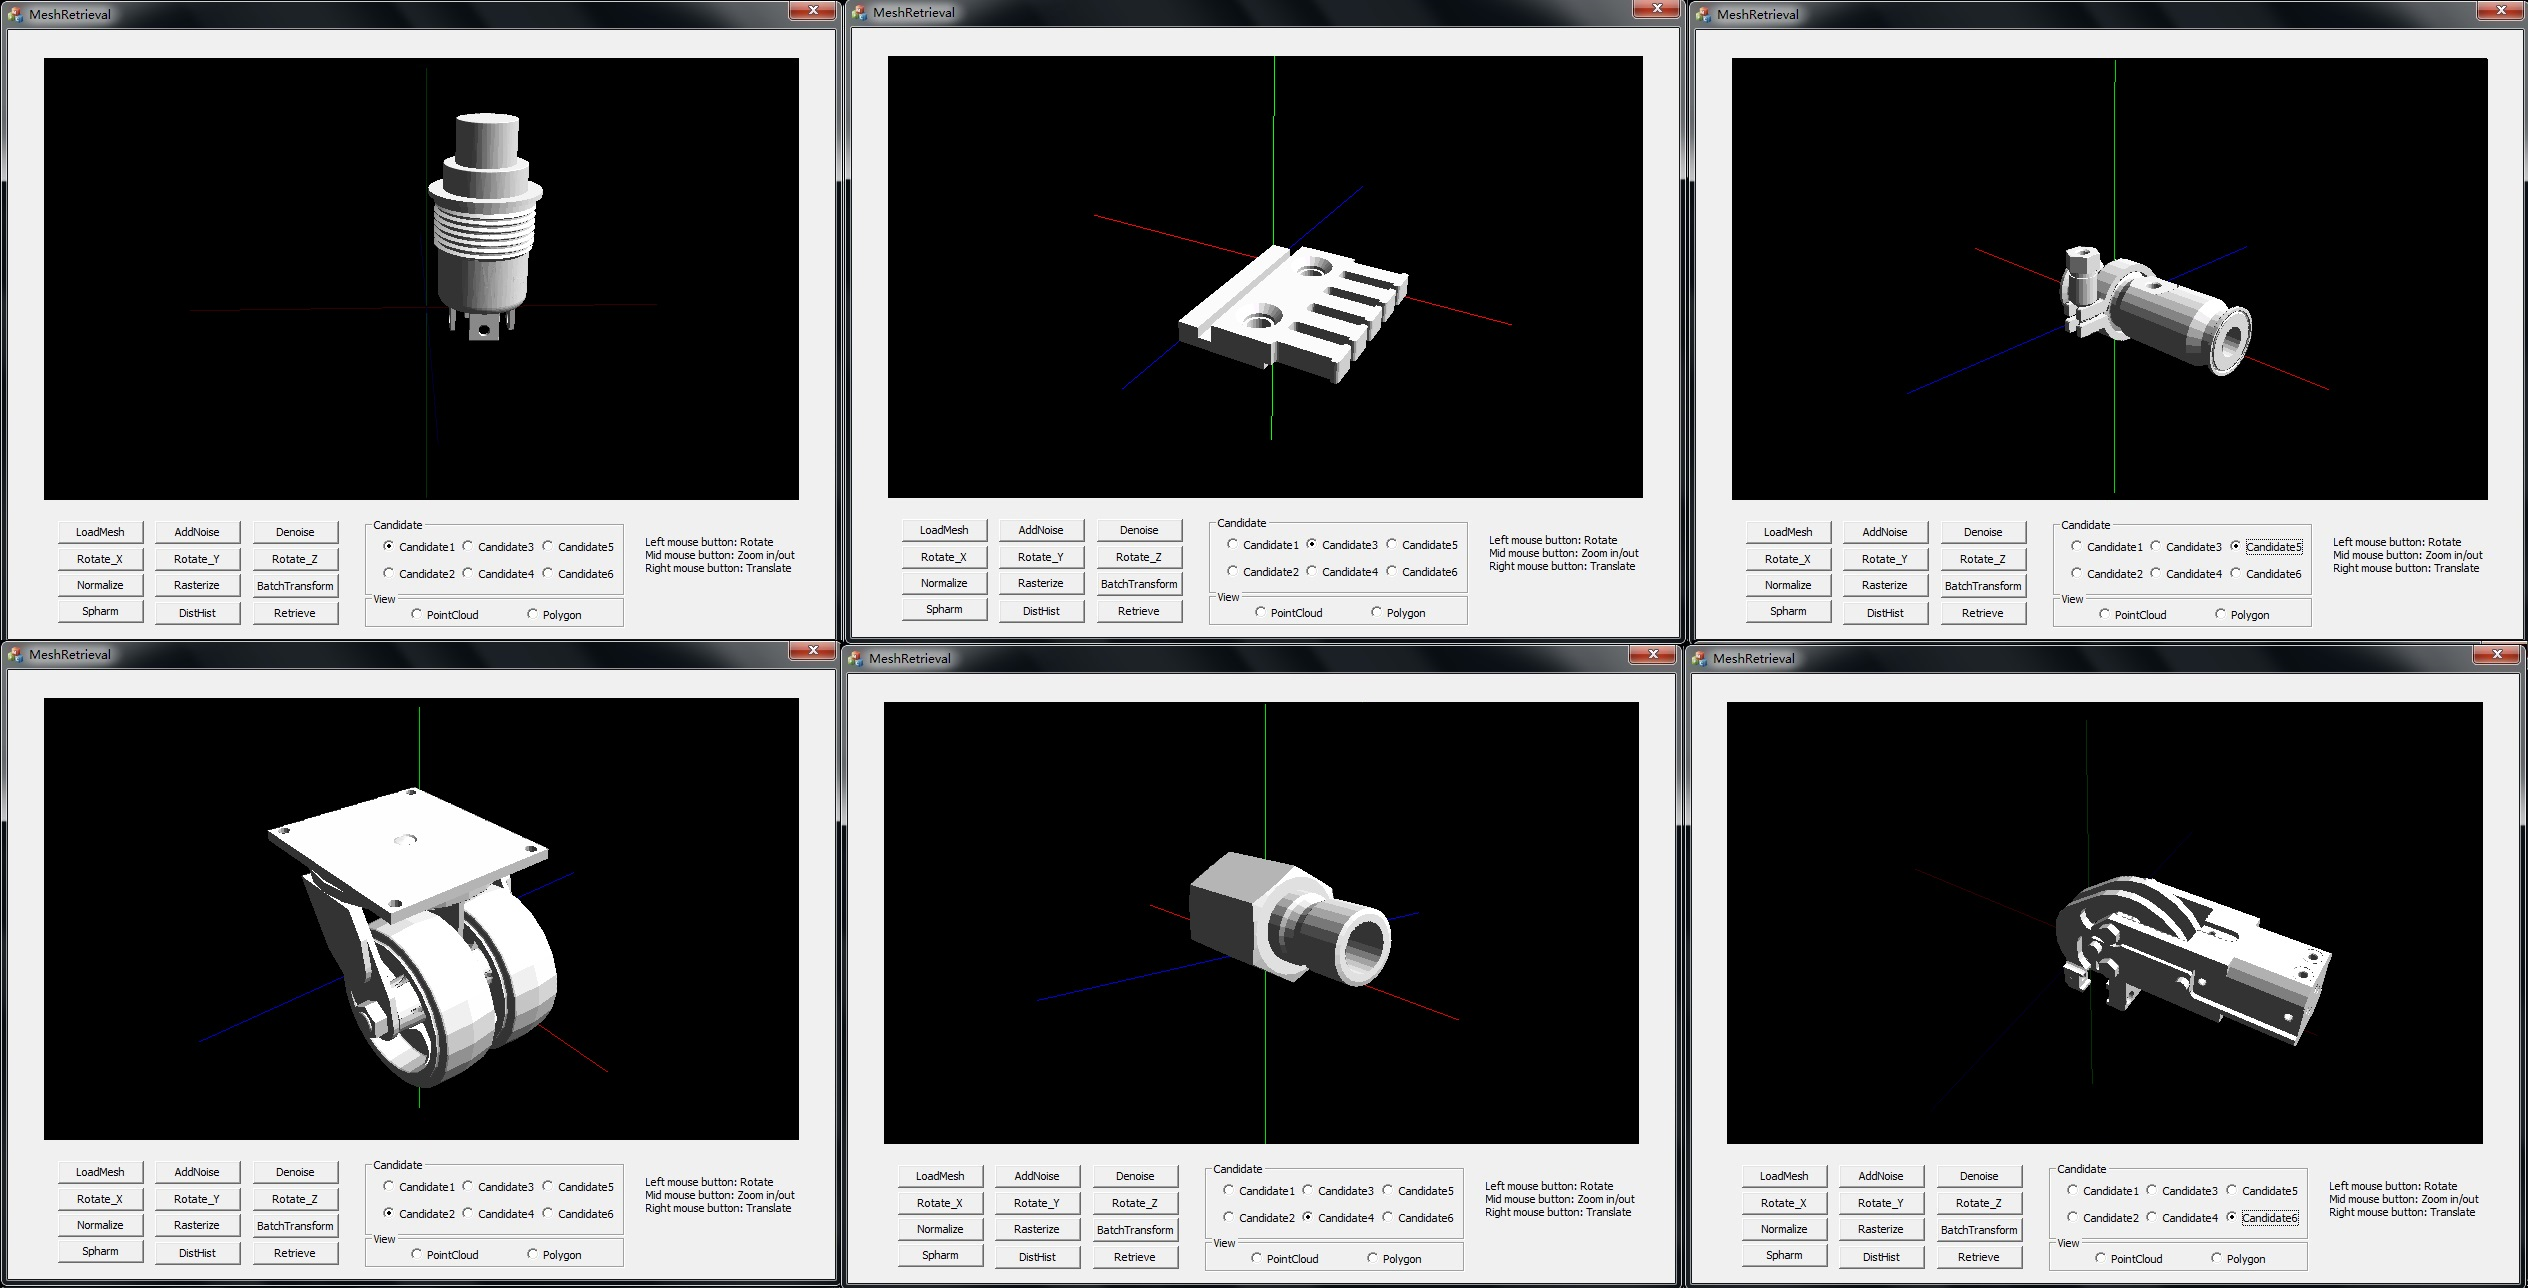
\includegraphics[width=1\linewidth]{output_noiseinvariant_test10}  \\
   (c)  \\
\caption{Noise resistant test: (a) the input model (noise added). (b) the input model (denoised). (c) the query result. It can be noticedthat the first candidate model has the same shape as the input model.} 
  \label{noiseinvarianttest_UI}
\end{center}
\end{figure}

\begin{figure}
\begin{center}
\begin{tabular}{cc}   % The "|" bar puts a bar in the figure
   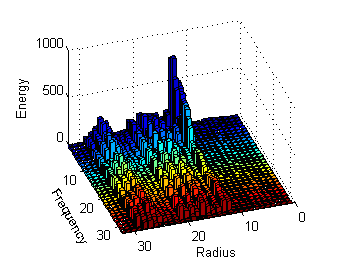
\includegraphics[width=0.45\linewidth]{noiseinvariant_test_SH10_denoise} & 
   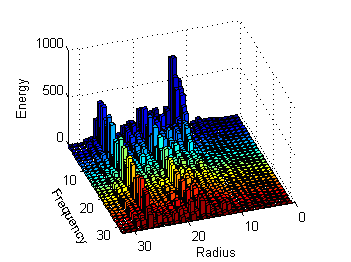
\includegraphics[width=0.45\linewidth]{noiseinvariant_test_SH10_origin}  \\
   (a) Spherical harmonics (noisy model) & (b) Spherical harmonics (origin model)\\
   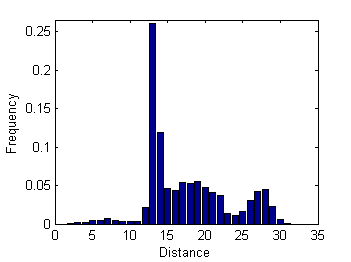
\includegraphics[width=0.45\linewidth]{noiseinvariant_test_DH10_denoise} &
   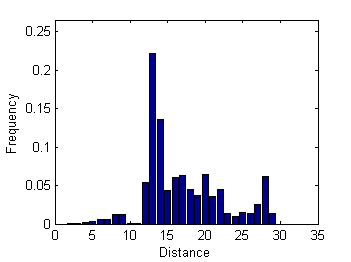
\includegraphics[width=0.45\linewidth]{noiseinvariant_test_DH10_origin}  \\
   (c) Distance histogram (noisy model) & (d) Distance histogram (origin model)\\
\end{tabular}
\caption{Analysis of the noise resistant test: Comparing with (a) and (b), (c) and (d), two types of the shape descriptors have similar features but only some slight changes. Therefore the noise resistant property of this system is verified. } 
  \label{noiseinvarianttest_analysis}
\end{center}
\end{figure}

\newpage

\begin{figure}
\begin{center}
\begin{tabular}{ccc}   % The "|" bar puts a bar in the figure
   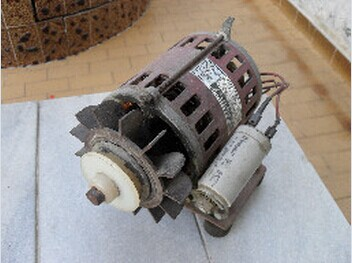
\includegraphics[height=0.23\columnwidth]{input_engine_photo_scantosearch_test}& 
   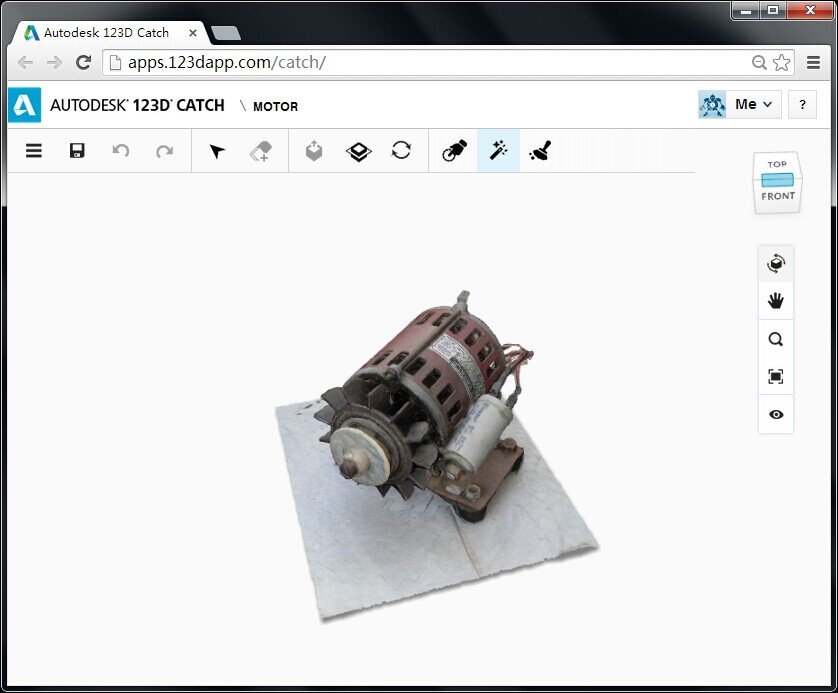
\includegraphics[height=0.23\columnwidth]{input_engine_rawscanned_scantosearch_test}&
   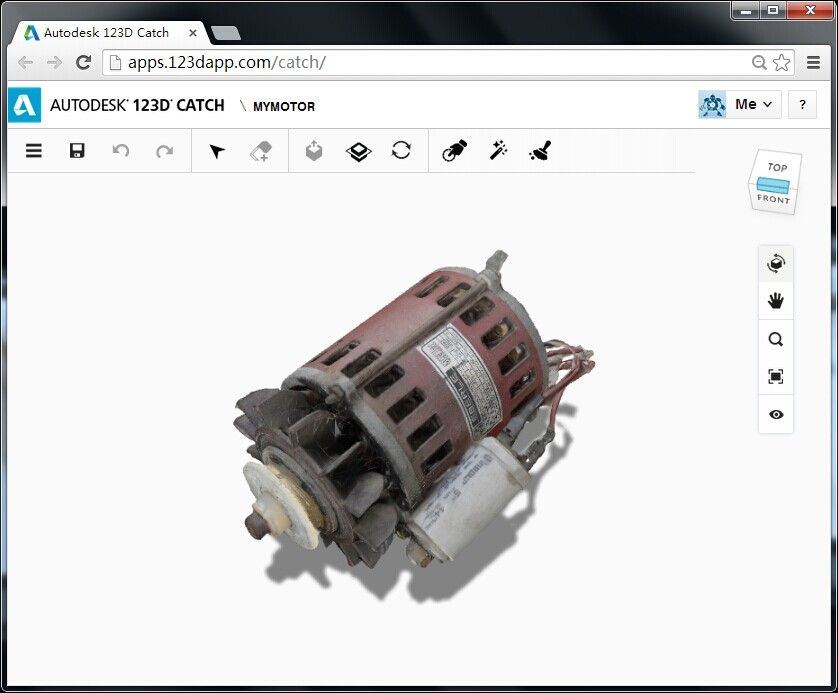
\includegraphics[height=0.23\columnwidth]{input_engine_scanned_scantosearch_test}\\
   (a) & (b) & (c)
\end{tabular}
\caption{``Scan to search'': (a) the engine. (b) the raw scanned model. (c) the processed model. The engine is scanned and its 3D model is created. } 
  \label{scantosearchtest_engine_scanning}
\end{center}
\end{figure}

\begin{figure}
\begin{center}
\begin{tabular}{c}   % The "|" bar puts a bar in the figure
   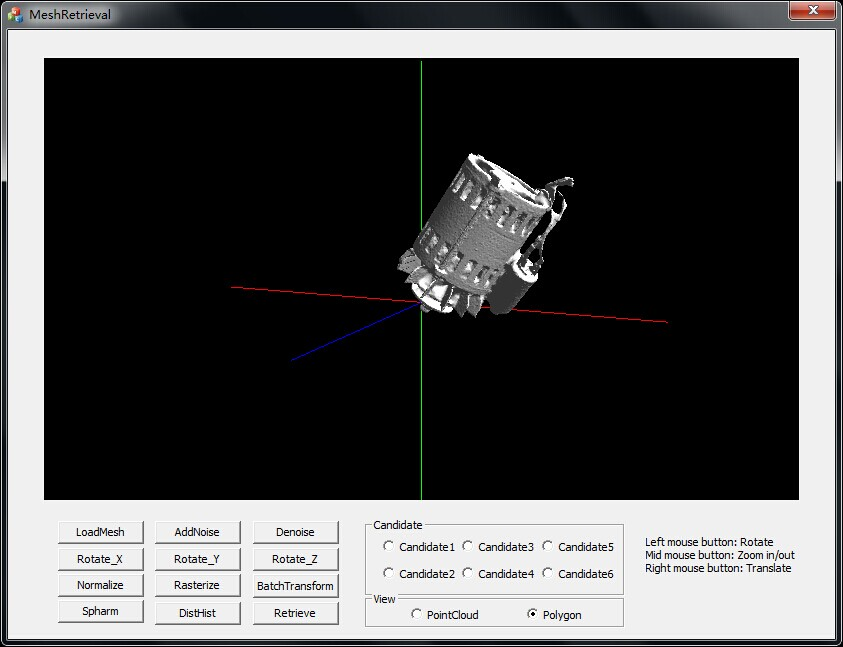
\includegraphics[height=0.4\columnwidth]{input_engine_scantosearch_test}\\
   (a)\\
   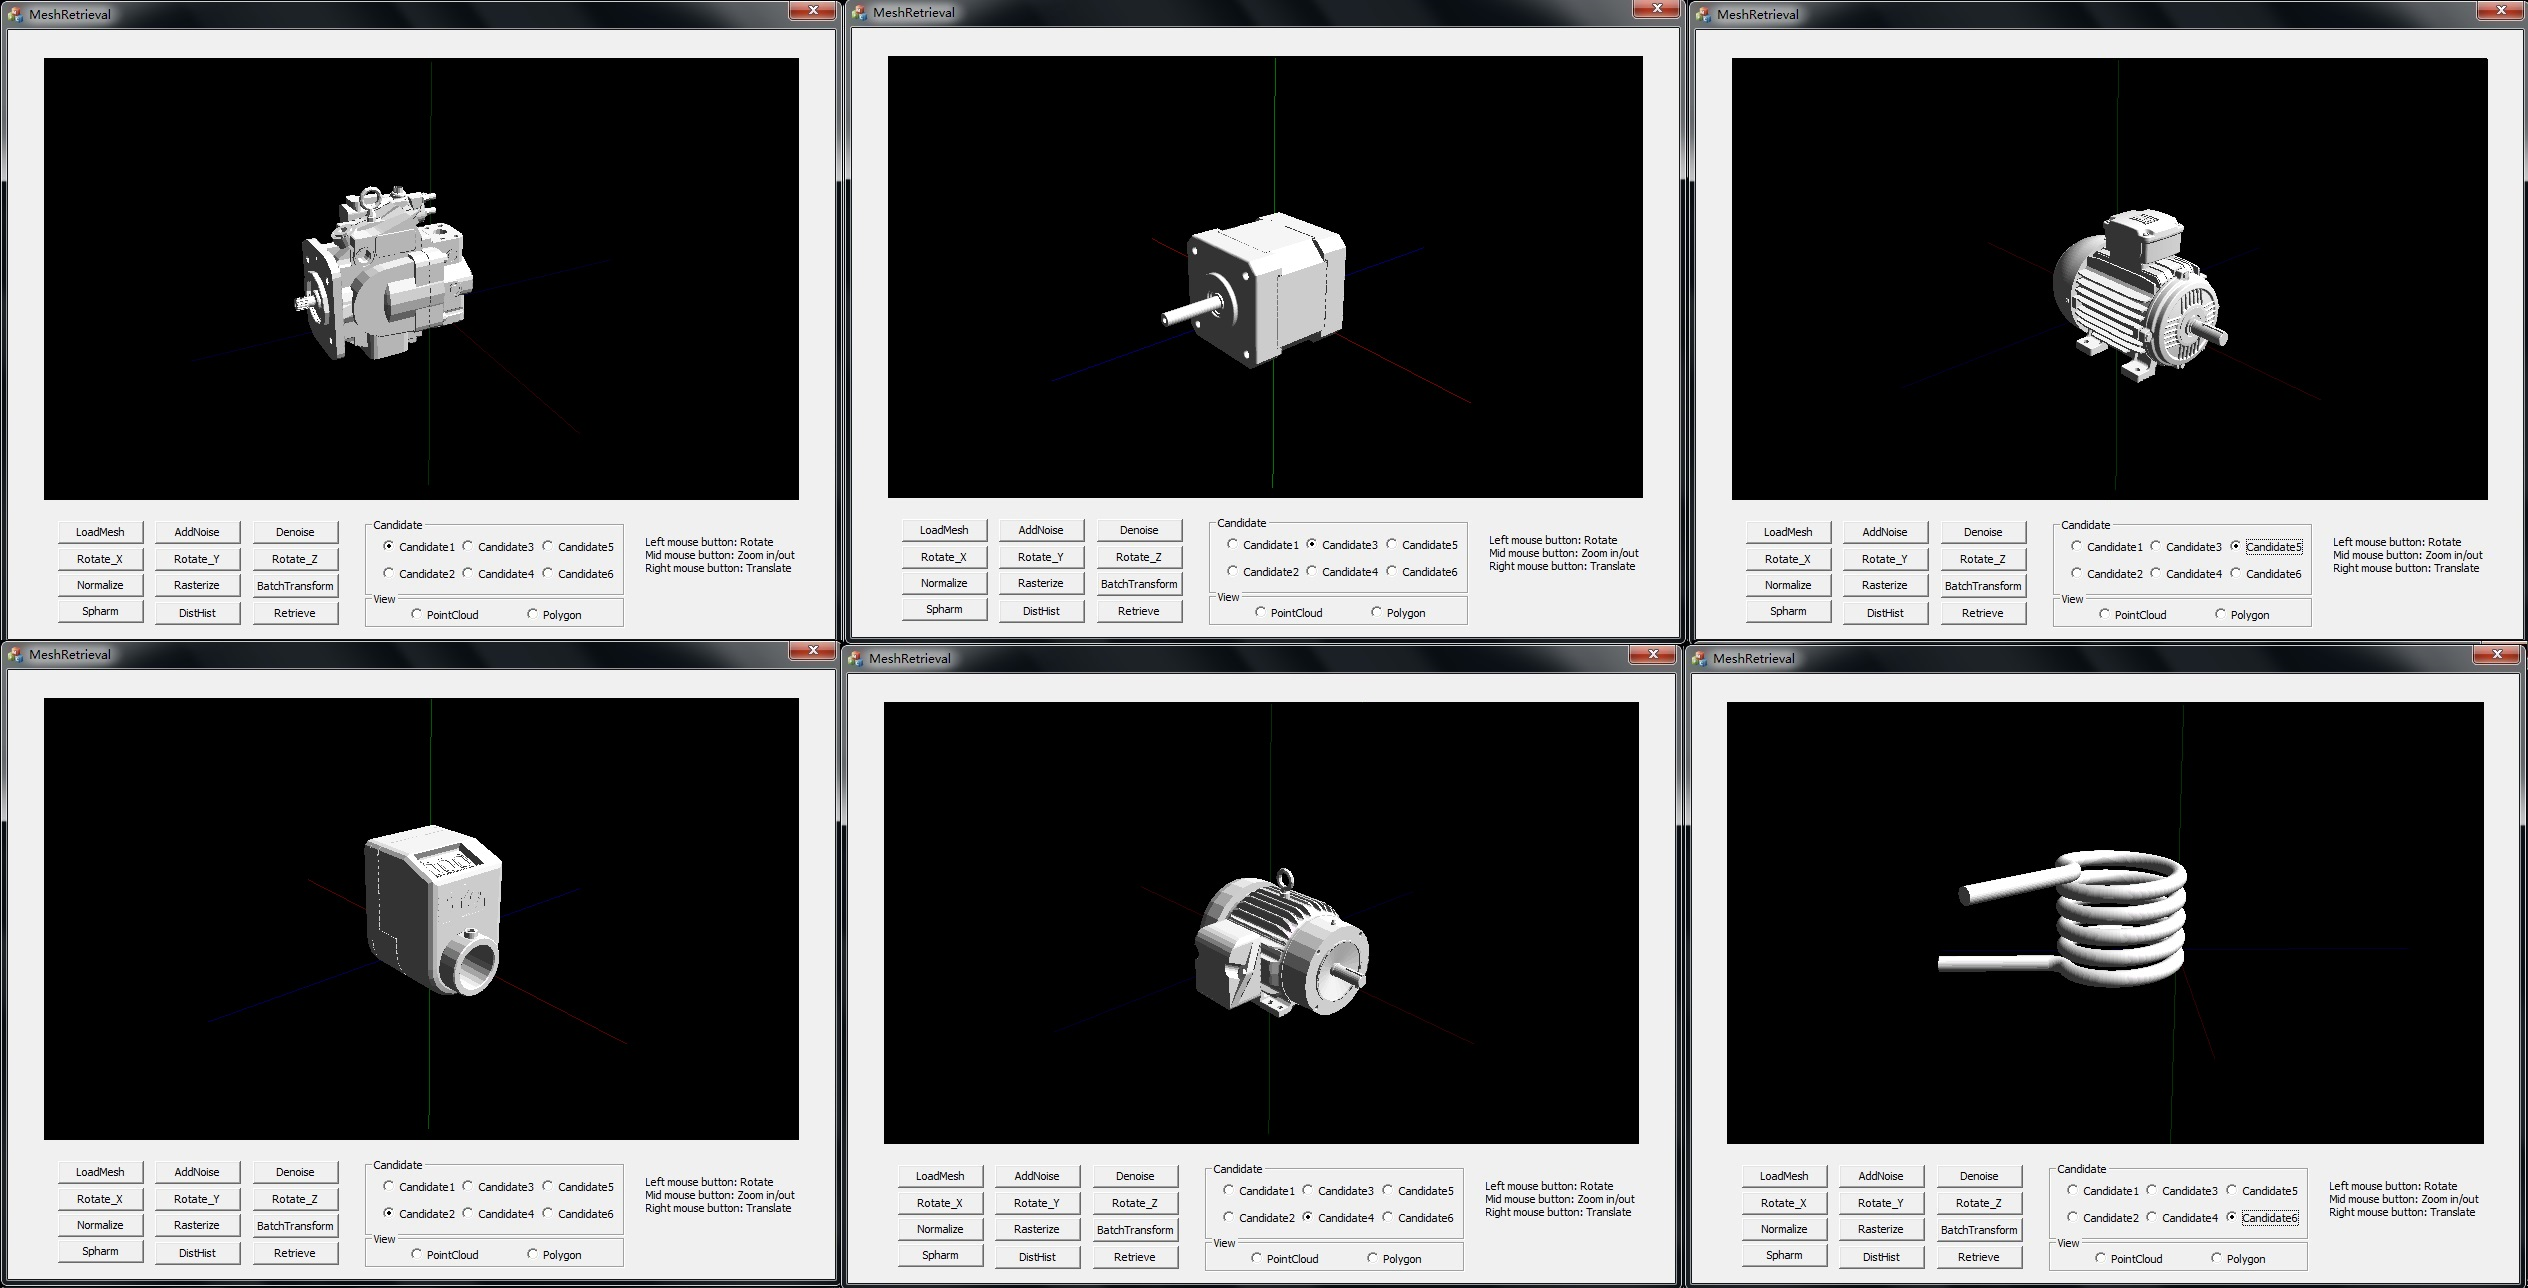
\includegraphics[width=0.95\linewidth]{output_engine_scantosearch_test}  \\
   (b)\\
\end{tabular}
\caption{``Scan to search'' test: (a) the scanned model. (b) query results.  Models with similar shapes are found. } 
  \label{scantosearchtest_engine_UI}
\end{center}
\end{figure}

\begin{figure}
\begin{center}
\begin{tabular}{ccc}   % The "|" bar puts a bar in the figure
   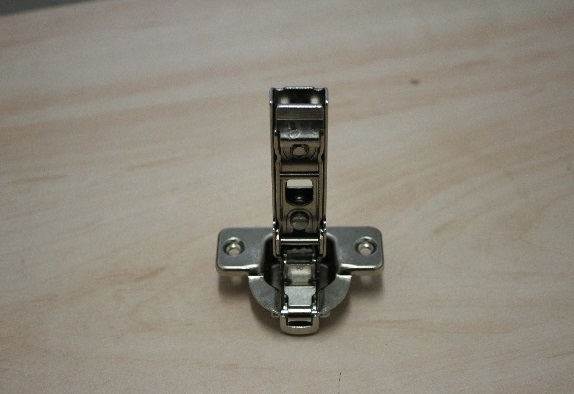
\includegraphics[height=0.23\columnwidth]{input_component_photo_scantosearch_test}& 
   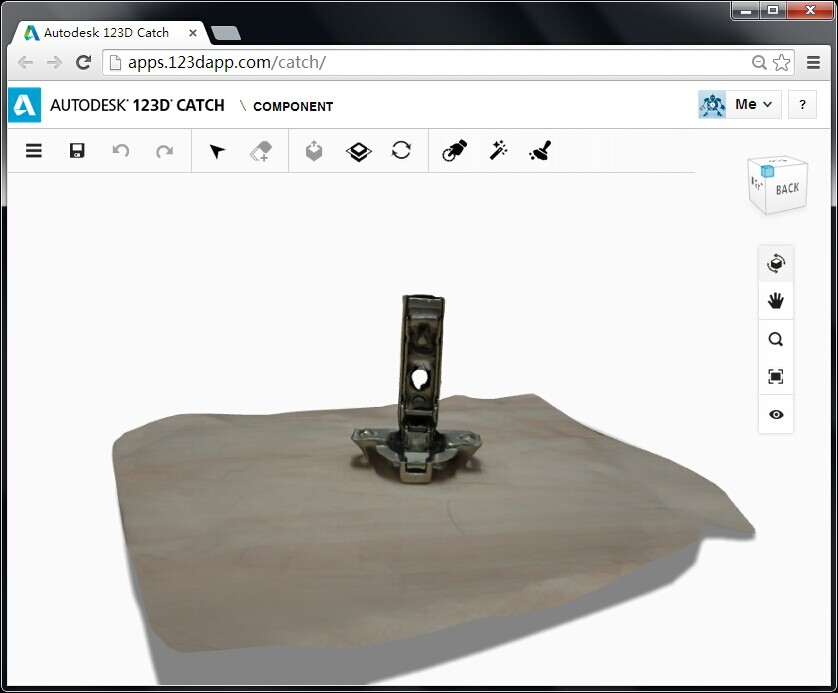
\includegraphics[height=0.23\columnwidth]{input_component_rawscanned_scantosearch_test}&
   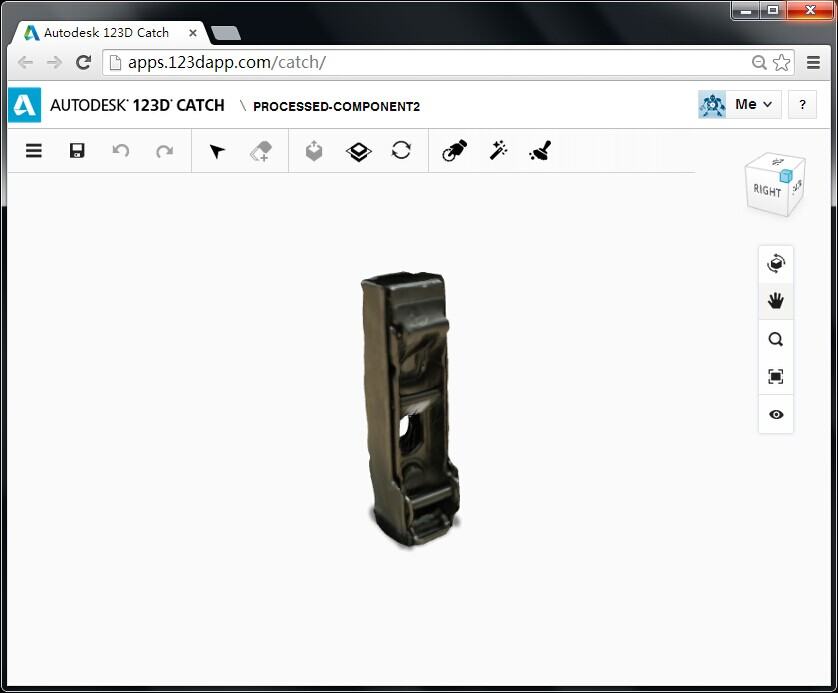
\includegraphics[height=0.23\columnwidth]{input_component_scanned_scantosearch_test}\\
   (a) & (b) & (c)
\end{tabular}
\caption{``Scan to search'': (a) the component. (b) the raw scanned model. (c) the processed model. The component is scanned and its 3D model is created. } 
  \label{scantosearchtest_component_scanning}
\end{center}
\end{figure}

\begin{figure}
\begin{center}
\begin{tabular}{c}   % The "|" bar puts a bar in the figure
   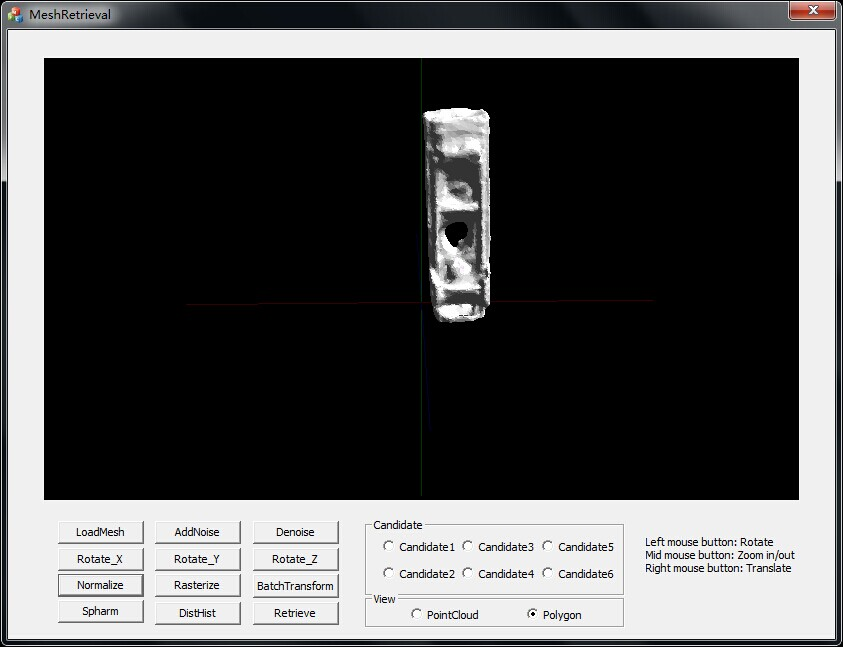
\includegraphics[height=0.4\columnwidth]{input_component_scantosearch_test}\\
   (a)\\
   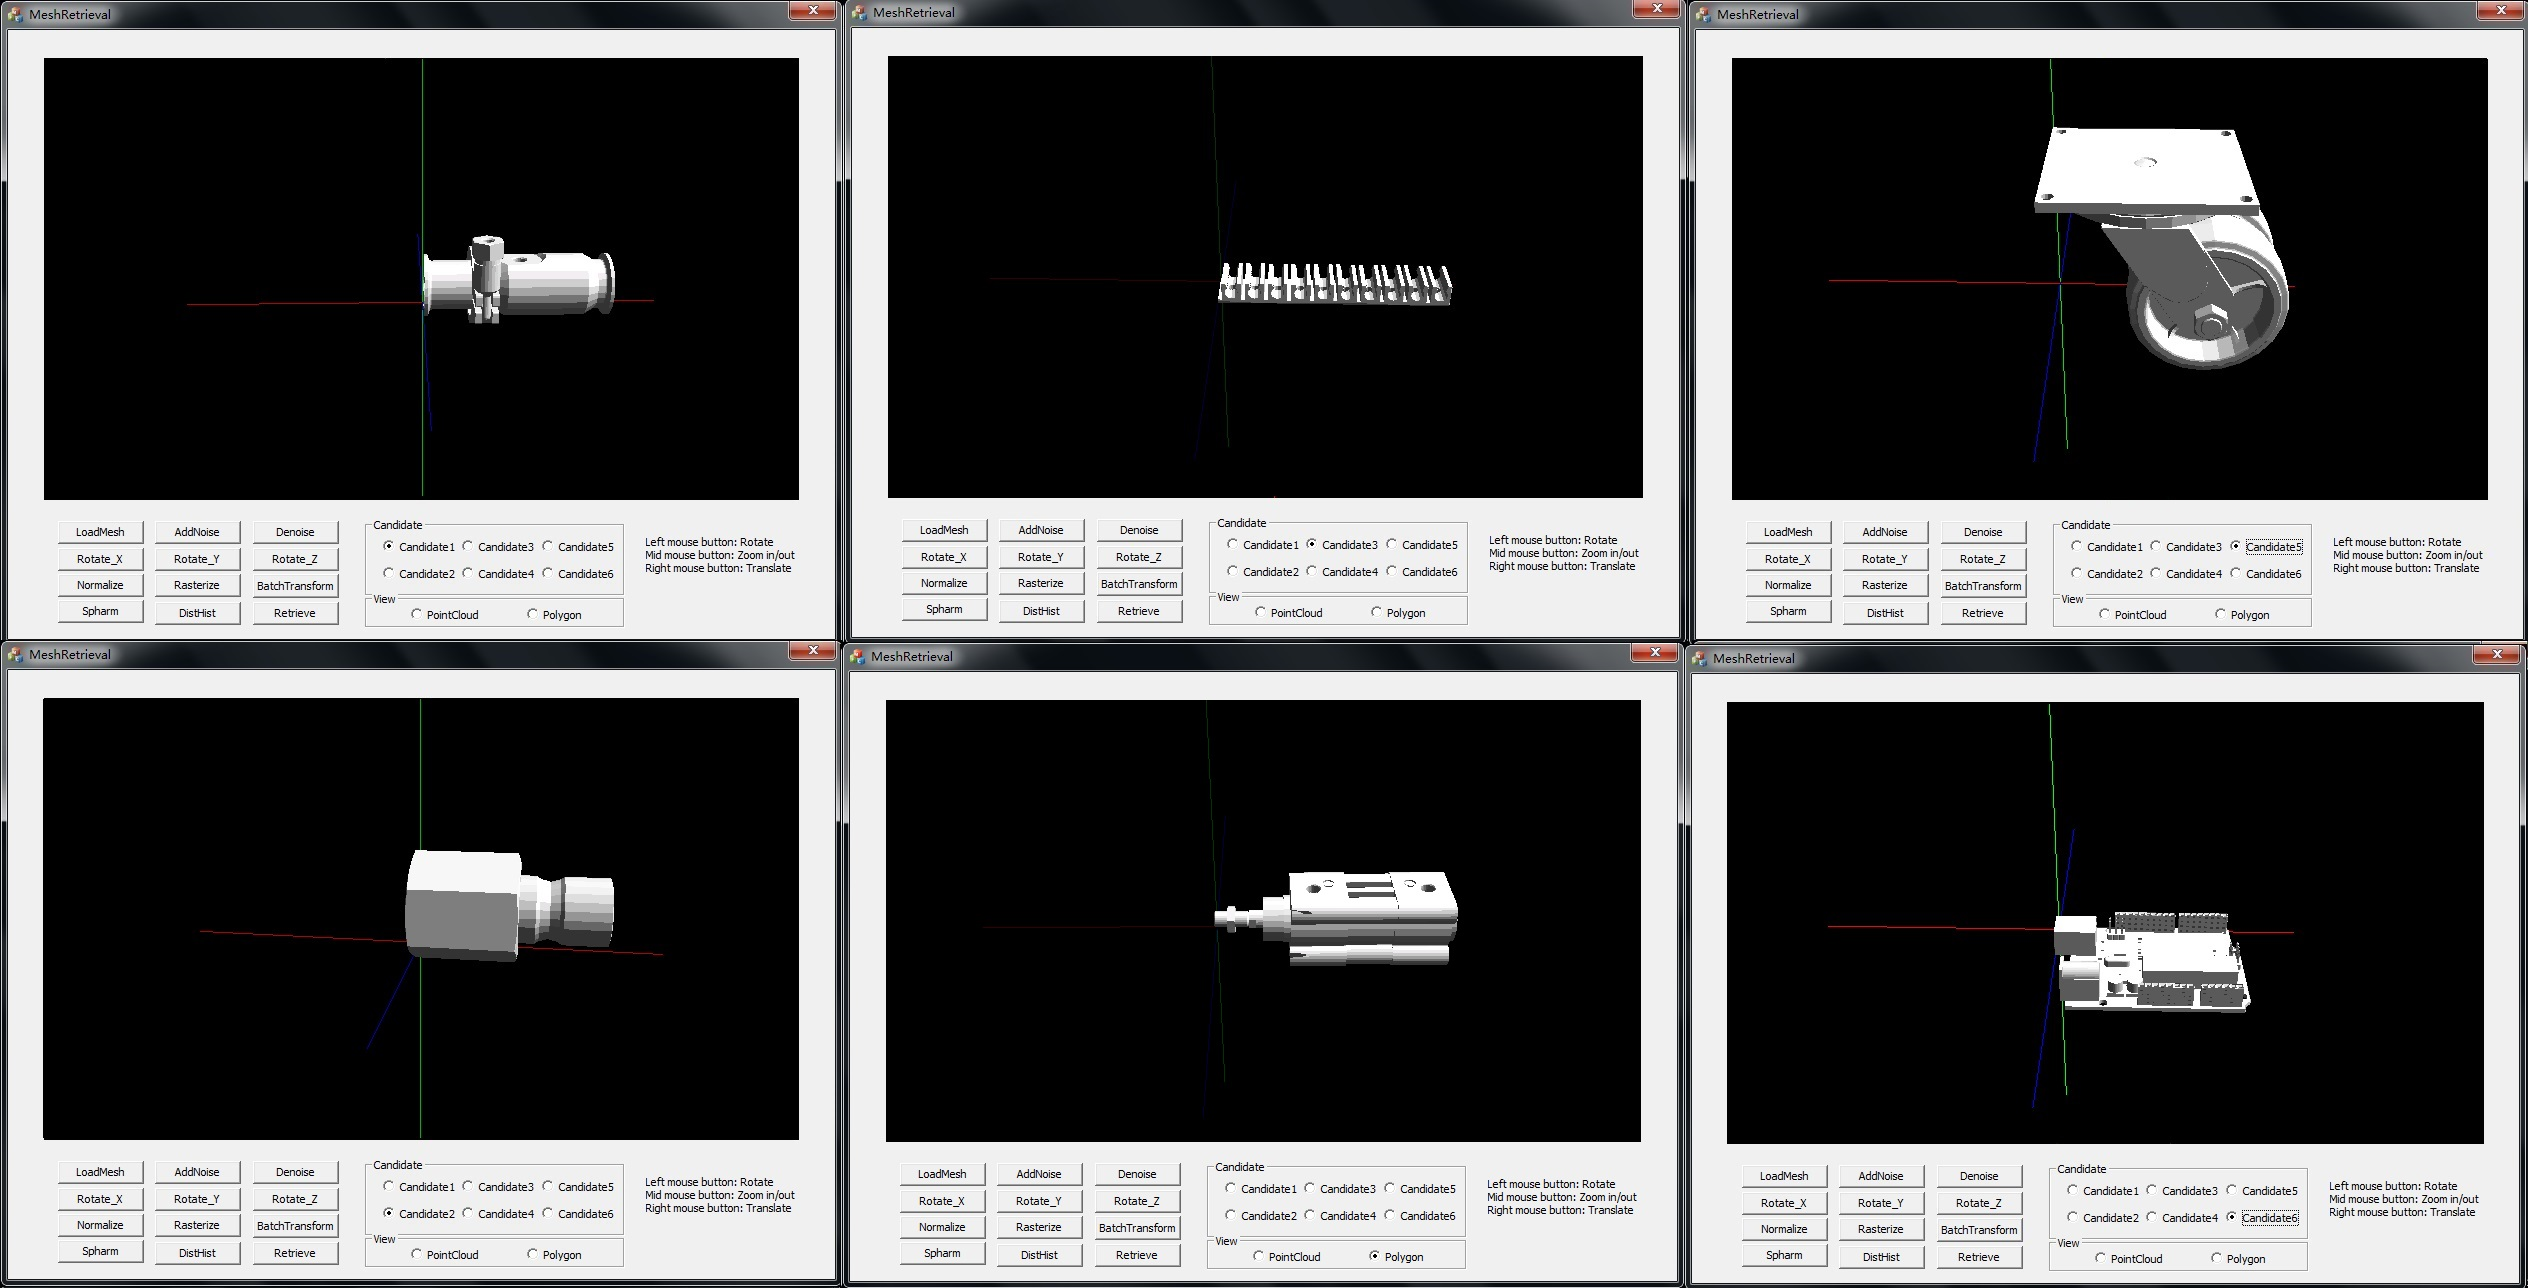
\includegraphics[width=0.95\linewidth]{output_component_scantosearch_test}  \\
   (b)\\
\end{tabular}
\caption{``Scan to search'' test: (a) the scanned model. (b) query results.  Models with similar shapes are found. } 
  \label{scantosearchtest_component_UI}
\end{center}
\end{figure}

\begin{figure}
\begin{center}
\begin{tabular}{ccc}   % The "|" bar puts a bar in the figure
   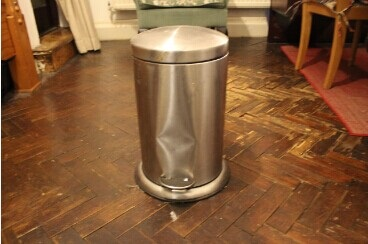
\includegraphics[height=0.23\columnwidth]{input_bin_photo_scantosearch_test}& 
   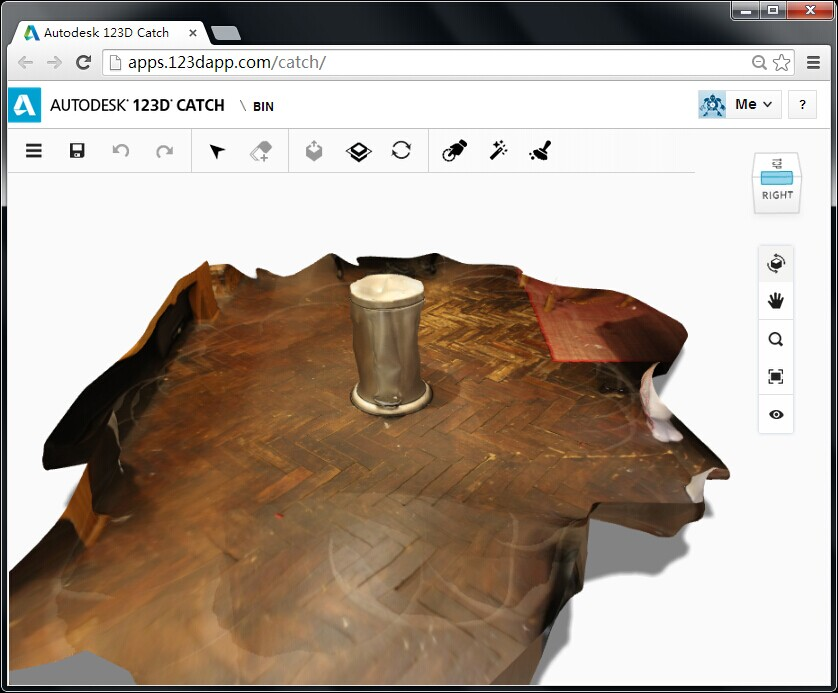
\includegraphics[height=0.23\columnwidth]{input_bin_rawscanned_scantosearch_test}&
   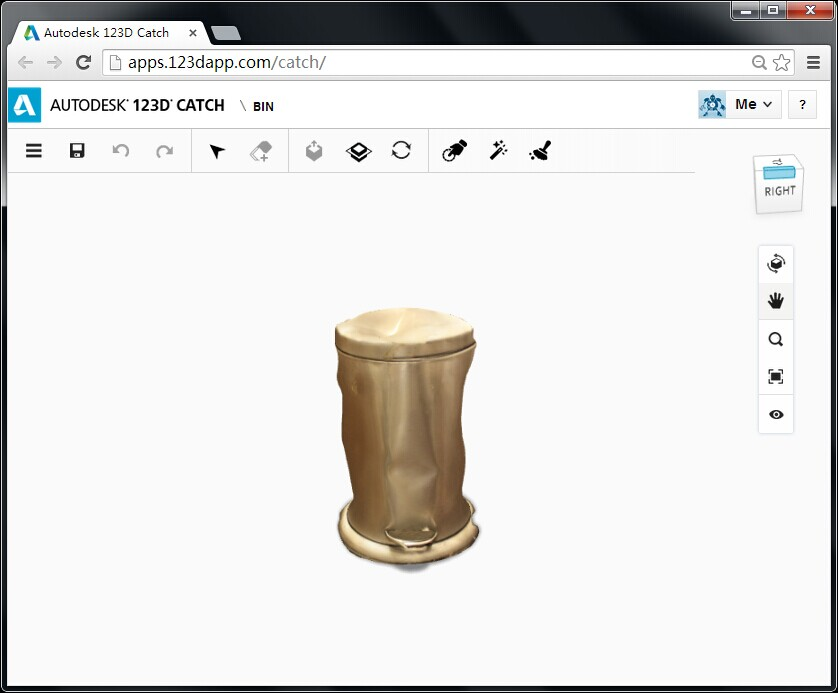
\includegraphics[height=0.23\columnwidth]{input_bin_scanned_scantosearch_test}\\
   (a) & (b) & (c)
\end{tabular}
\caption{``Scan to search'': (a) the bin. (b) the raw scanned model. (c) the processed model. The bin is scanned and its 3D model is created. } 
  \label{scantosearchtest_bin_scanning}
\end{center}
\end{figure}

\begin{figure}
\begin{center}
\begin{tabular}{c}   % The "|" bar puts a bar in the figure
   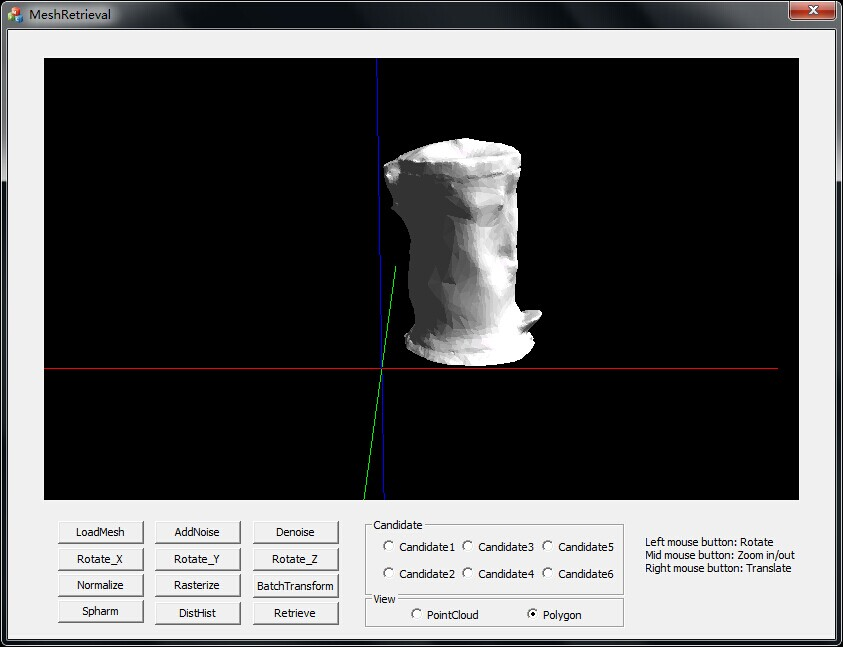
\includegraphics[height=0.4\columnwidth]{input_bin_scantosearch_test}\\
   (a)\\
   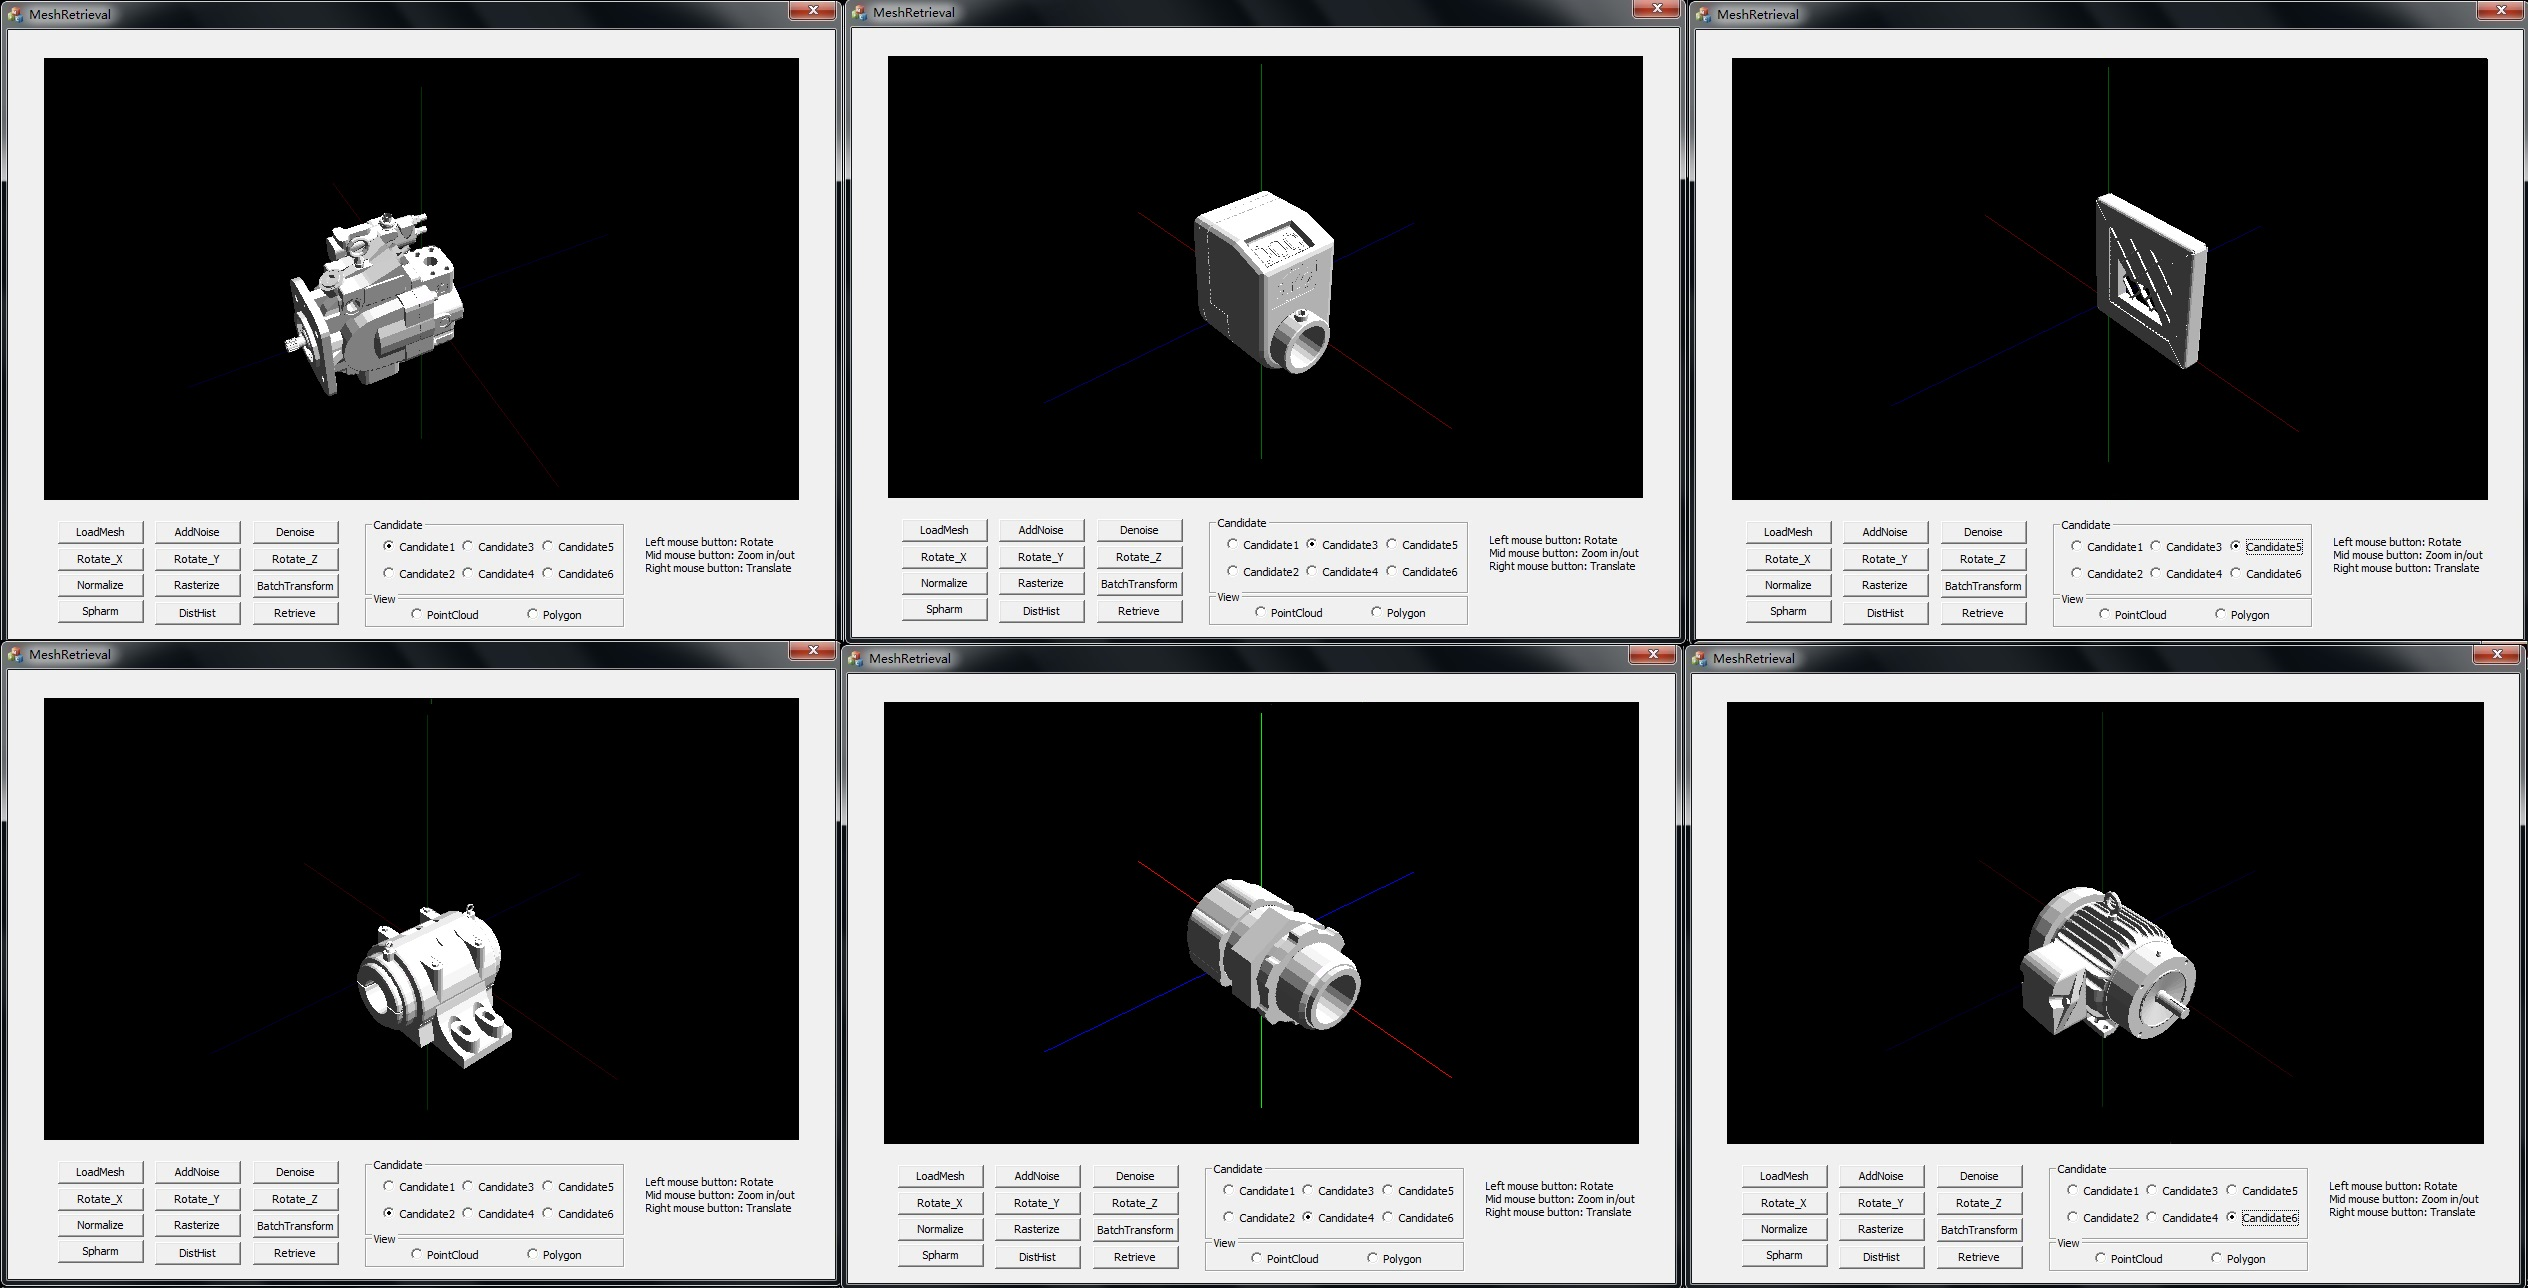
\includegraphics[width=0.95\linewidth]{output_bin_scantosearch_test}  \\
   (b)\\
\end{tabular}
\caption{``Scan to search'' test: (a) the scanned model. (b) query results.  Models with similar shapes are found. } 
  \label{scantosearchtest_bin_UI}
\end{center}
\end{figure}

\begin{figure}
\begin{center}
\begin{tabular}{ccc}   % The "|" bar puts a bar in the figure
   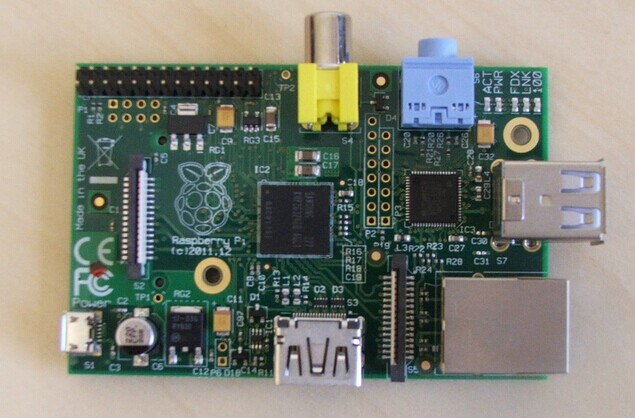
\includegraphics[height=0.23\columnwidth]{input_pi_photo_scantosearch_test}& 
   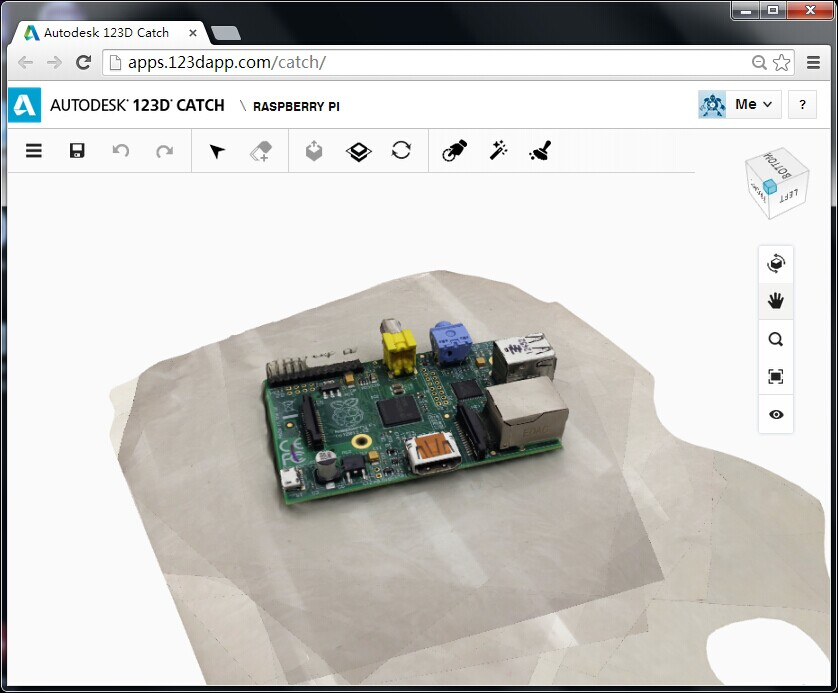
\includegraphics[height=0.23\columnwidth]{input_pi_rawscanned_scantosearch_test}&
   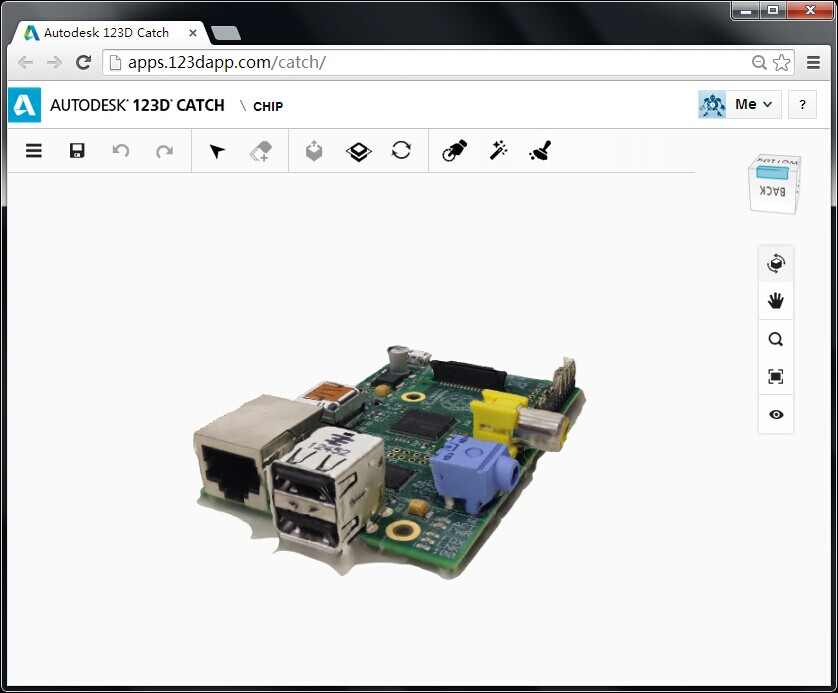
\includegraphics[height=0.23\columnwidth]{input_pi_scanned_scantosearch_test}\\
   (a) & (b) & (c)
\end{tabular}
\caption{``Scan to search'': (a) the single-board computer. (b) the raw scanned model. (c) the processed model. The component is scanned and its 3D model is created. } 
  \label{scantosearchtest_pi_scanning}
\end{center}
\end{figure}

\begin{figure}
\begin{center}
\begin{tabular}{c}   % The "|" bar puts a bar in the figure
   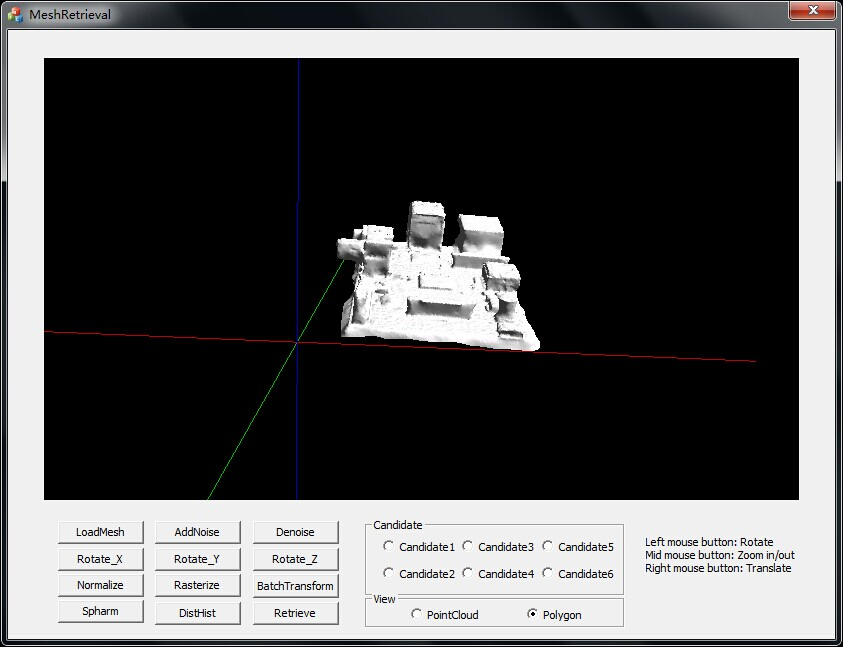
\includegraphics[height=0.4\columnwidth]{input_pi_scantosearch_test}\\
   (a)\\
   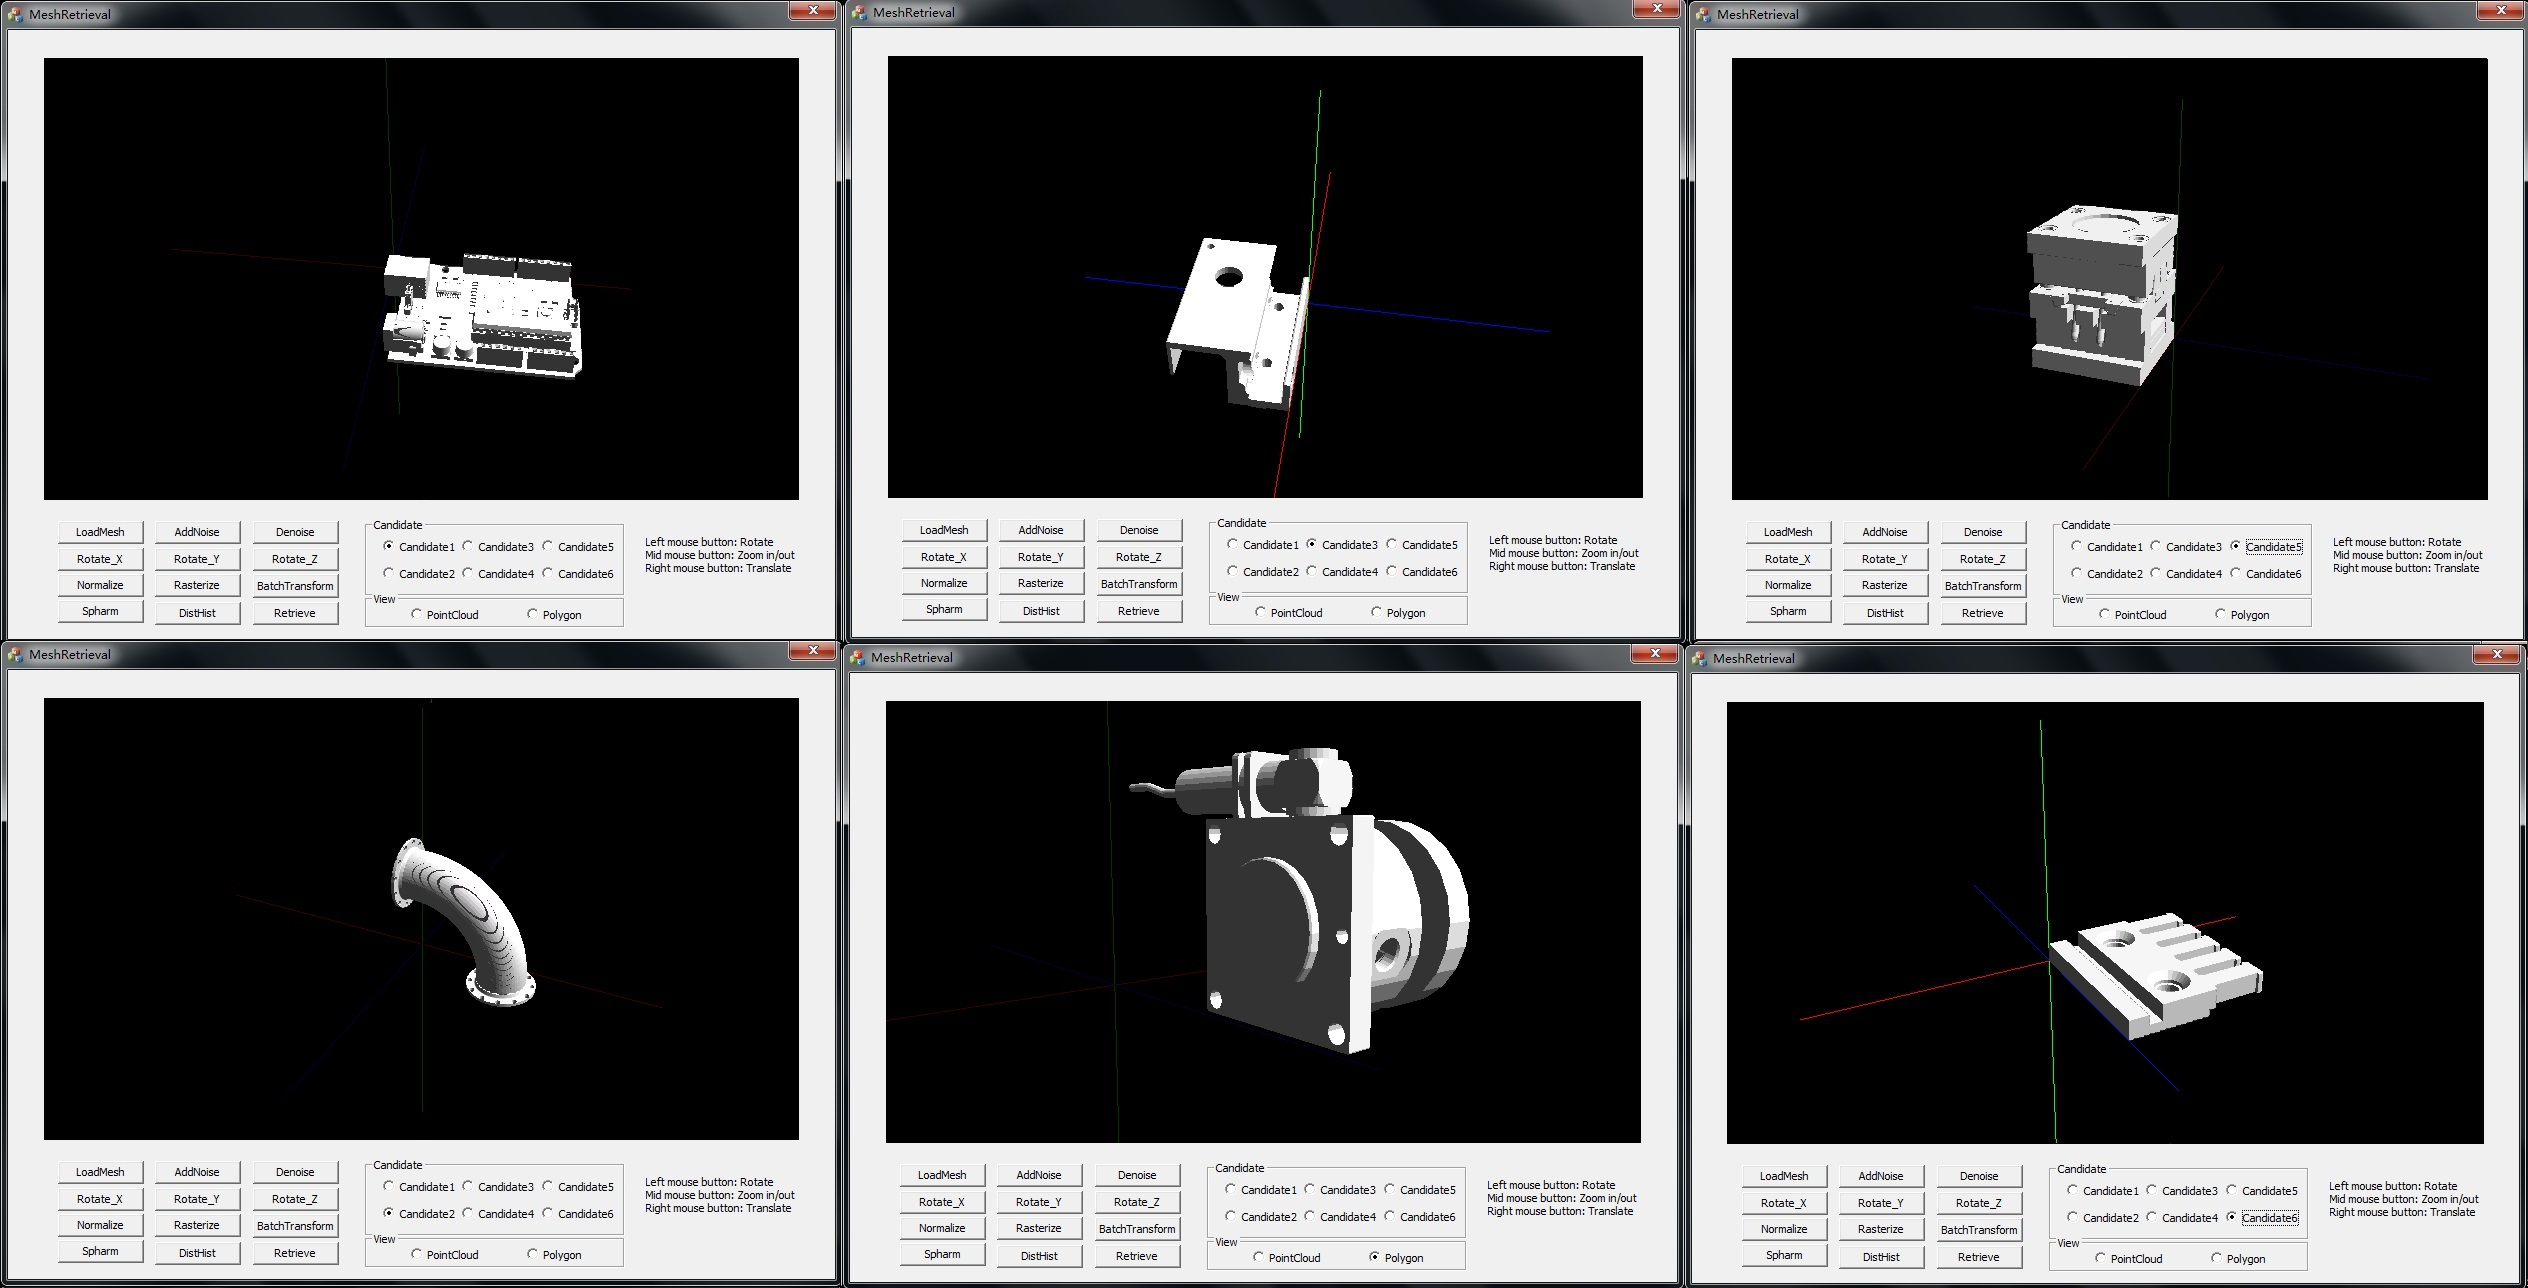
\includegraphics[width=0.95\linewidth]{output_pi_scantosearch_test}  \\
   (b)\\
\end{tabular}
\caption{``Scan to search'' test: (a) the scanned model. (b) query results.  Models with similar shapes are found. } 
  \label{scantosearchtest_pi_UI}
\end{center}
\end{figure}
%example for subfigure
%\begin{figure}
%    \begin{subfigure}[b]{.45\linewidth}
%        \centering
%            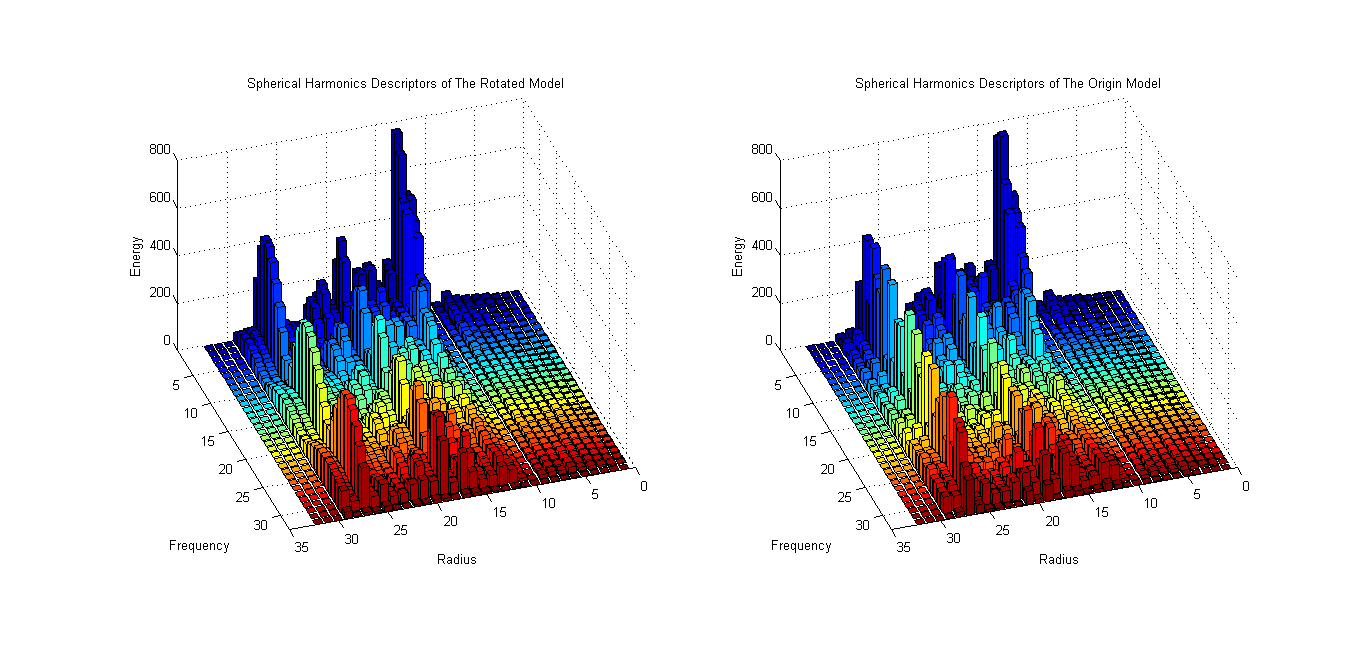
\includegraphics[scale=.3]{rotationinvariant_test_SH10}
%            \caption{Skeletal}
%        \label{fig:SkeletalTissue}
%    \end{subfigure}
%    \begin{subfigure}[b]{.45\linewidth}
%        \centering
%            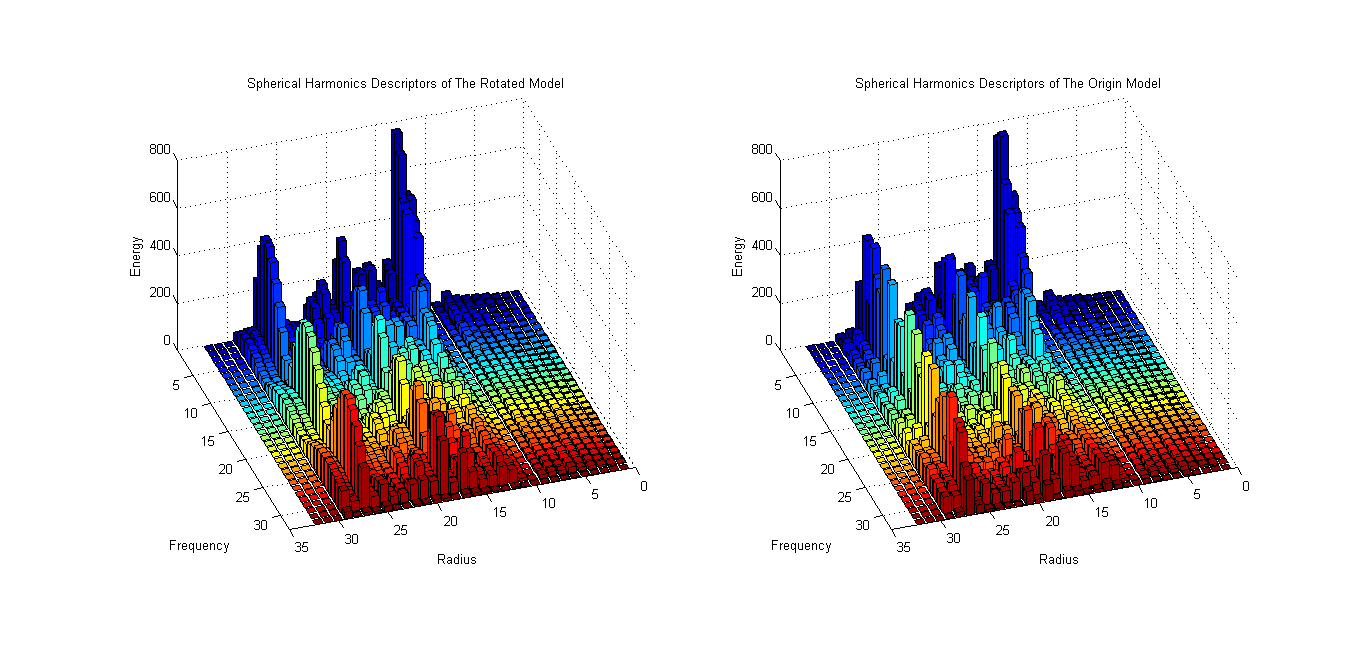
\includegraphics[scale=.3]{rotationinvariant_test_SH10}
%            \caption{Cardiac}
%        \label{fig:CardiacTissue}
%    \end{subfigure}
%    \caption{Types of Muscular Tissue}
%    \label{fig:MuscularTissue}
%\end{figure}

